\documentclass[11pt]{article}   % list options between brackets
%\usepackage{}              % list packages between braces
\usepackage{amsmath}
\usepackage{mathtools}
\usepackage{graphicx}
\usepackage{verbatim}
\usepackage{multirow}

\setlength{\textwidth}{15.5cm}
\setlength{\oddsidemargin}{1.0cm}
\setlength{\evensidemargin}{1.0cm}
\setlength{\textheight}{21.0cm}
\setlength{\footskip}{1.0cm}
%\setlength\parindent{0pt}

\begin{document}

\title{MetReader: Documentation and User's Guide}   % type title between braces
\author{Hans F. Schwaiger}
\date{June 1, 2023}    % type date between braces
\maketitle

%%%%%%%%%%%%%%%%%%%%%%%%%%%%%%%%%%%%%%%%%%%%%%%%%%%%%%%%%%%%%%%%%%%%%%%%%%%%%%%
\section{Introduction}
MetReader is a library written in fortran 90 that provides an interface to
numerical weather prediction (NWP) data, or other forms of meteorological
data, such as radiosonde or other 1-D data.

This library was originally written as a component of the USGS volcanic ash
transport and dispersion model, Ash3d.  However, since it is useful for
programs other than Ash3d, this interface to NWP files is provided
as a separate repository that can either be compiled as a library or simply
compiled directly with other source code.

NWP data are generally made available by agencies (NCEP, NOAA, NASA, etc.)
in a variety of formats (NetCDF, GRIB, ASCII); each product having
its own data structure, naming convention, units, etc.  This library
isolates the calling program from the peculiarities of interfacing with
a particular NWP product.  Data can be returned to the calling program on
the native grid of the NWP product, or on any grid needed by the calling
program.  Projection and interpolation of NWP data to the required grid, along
with any rotation of velocity vectors to grid-relative, is calculated internally by
MetReader.

%%%%%%%%%%%%%%%%%%%%%%%%%%%%%%%%%%%%%%%%%%%%%%%%%%%%%%%%%%%%%%%%%%%%%%%%%%%%%%%
\section{Installation}
This library requires two additional libraries made available on GitHub and USGS GitLab:
\begin{itemize}
\item HoursSince \\
This is a library that takes a date and time, and calculates the number of hours
since January 1, 1900 (or any arbitrary base year).\\
(https://github.com/DOI-USGS/volcano-ash3d-hourssince)
\item projection \\
This is a library that calculates commonly-used projected coordinates.\\
(https://github.com/DOI-USGS/volcano-ash3d-projection)
\end{itemize}

These libraries are installed by default into \texttt{/opt/USGS}.  If they are
installed elsewhere, then you will need to edit the \texttt{makefile}
to point to your installation.
Additionally, the default \texttt{makefile} will build MetReader with both NetCDF and GRIB
interfaces enabled.  If either of these libraries are unavailable on your system, you can
deactivate those options by setting the corresponding flags to \texttt{F} in the makefile.
On a Redhat systems (Fedora, RHEL, CentOS, Rocky), you can install the data
format libraries by typing
\begin{verbatim}
     sudo yum install netcdf netcdf-devel netcdf-fortran netcdf-fortran-devel
     sudo yum install eccodes eccodes-devel
\end{verbatim}
or for Ubuntu
\begin{verbatim}
     sudo apt-get install libnetcdf* libgrib-api*
\end{verbatim}
To compile MetReader as a library, simply type:
\begin{verbatim}
     make lib
\end{verbatim}
This will build the requested components of the library.  If \texttt{GRIB} is enabled,
this will also build the GRIB indexer, \texttt{gen\_GRIB\_index}.
This is a tool that generates an index file of the GRIB records which speeds
access time to individual records substantially.
Several other tools can be build via the command:
\begin{verbatim}
     make tools
\end{verbatim}
These tools include the following (described in Sec. \ref{SecTools}).
\begin{itemize}
\item \texttt{MetRegrid} : This program reads a variable from a NWP file and regrids\
the data to a user-specified grid; then write out regridded point, line, sheet, or volume data.
\item \texttt{MetSonde} : This tool takes command-line arguments specifying date, time, location
and writes a file with temperature vs height from GFS or NCEP data.
\item \texttt{MetCheck} : This program tests the windfiles to make sure all variable values
are within the expected ranges.
\item \texttt{gen\_GRIB\_index} : This tool builds a grib index to facilitate reading of grib
files.
\item \texttt{MetProbe} : This is a more general version of \texttt{MetSonde} controled by
an input file that can handle more NWP data types.
\item \texttt{MetTraj\_F} : This tool will generate foreward trajectories from based on the
time-series NWP data.
\item \texttt{MetTraj\_B} : This tool will generate backward trajectories from based on the
time-series NWP data.
\item \texttt{makegfsncml} :  This tool is used to strip out unused variable when converting
grib to netCDF using the download scripts.
\end{itemize}

To test the build, type:
\begin{verbatim}
     make check
\end{verbatim}
This will run three tests using the radiosonde data (found in \texttt{examples/UpperAirSoundings}),
followed by three tests using the NCEP 50-year reanalysis data.  The three test for
each wind data type are: \texttt{MetProbe}, \texttt{MetTraj\_F}, and \texttt{MetRegri}.
Output data file are compared with saved datafiles in \texttt{tests/output*}. Note that
the files are only compared using the unix \texttt{cmp} command and small differences
can be present in output files depending on if \texttt{OPT} or \texttt{DEBUG} was used
when building the tools.

To install the library, module files and tools, edit the \texttt{INSTALLDIR} variable of
the makefile (the default is \texttt{/opt/USGS}) and type:
\begin{verbatim}
     make all
     make install
\end{verbatim}
This will also install scripts that can be used to download the $0.5^{\circ}$ GFS
forecast files and the NCEP $2.5^{\circ}$ Reanalysis files.

You will need to have write permission in \texttt{\$\{INSTALLDIR\}}
or install as root.  Assuming the libraries \texttt{projection} and \texttt{hourssince} are
installed in the default location, installation will result in the following
directory structure:
\begin{verbatim}
/opt/USGS
|-- bin
|   |-- autorun_scripts
|   |   |-- autorun_gfs0.5deg.sh
|   |   |-- autorun_NCEP_50YearReanalysis.sh
|   |   |-- convert_gfs0.5deg.sh
|   |   |-- get_gfs0.5deg.sh
|   |   |-- get_NCEP_50YearReanalysis.sh
|   |   `-- grib2nc.sh
|   |-- gen_GRIB_index
|   |-- HoursSince1900
|   |-- MetCheck
|   |-- MetRegrid
|   |-- MetSonde
|   |-- MetTraj_B
|   |-- MetTraj_F
|   |-- MetProbe
|   |-- project_for
|   |-- project_inv
|   `-- yyyymmddhh_since_1900
|-- include
|   |-- metreader.mod
|   `-- projection.mod
`-- lib
    |-- libhourssince.a
    |-- libMetReader.a
    `-- libprojection.a
\end{verbatim}

The \texttt{makefile} included the following variables that can be changed, depending on your
system.
\begin{itemize}
\item \texttt{SYSTEM} : \texttt{gfortran} or \texttt{ifort}\\
Fortran compiler.
\item \texttt{RUN} : \texttt{DEBUG}, \texttt{PROF} or \texttt{OPT}\\
Sets class of compiler flags for debugging, profiling, of optimization:
\item \texttt{INSTALLDIR} : \texttt{/opt/USGS} \\
Install location.
\item \texttt{USENETCDF} : \texttt{T} or \texttt{F}\\
Logical flag to build netCDF interface.
\item \texttt{USEGRIB} : \texttt{T} or \texttt{F}\\
Logical flag to build GRIB2 interface.
\item \texttt{USEPOINTERS} : \texttt{T} or \texttt{F}\\
Logical flag to define public work arrays as pointer or allocatable space. There is no
real proformance impact for either choice. Older \texttt{gfortran} compilers
required allocatable arrays, but pointers facilitate access from \texttt{C} programs.
\end{itemize}

\clearpage
%%%%%%%%%%%%%%%%%%%%%%%%%%%%%%%%%%%%%%%%%%%%%%%%%%%%%%%%%%%%%%%%%%%%%%%%%%%%%%%
\section{Usage}
MetReader can read a variety of input data formats (1-D, 3-D, ASCII, NetCDF, GRIB) and
provide access to the meteorological data on either the native grid of the NWP data, or interpolated
onto a finer regular grid.  Before the meteorological data can be accessible, several preliminary steps
must first be completed.
%%%%%%%%%%%%%%%%%%%%%%%%%%%%%%%%%%%%%%%%%%%%%%%%%%%%%%%%%%%
\subsection{Preliminary meta-data}\label{SSecPrelimMetaData}
The calling program needs to prepare several parameters that define the type of meteorological
data to be read.  
\begin{itemize}
\item \texttt{iw} :: windfile class 
 \begin{itemize}
 \item 1 : 1-D wind sounding
 \item 2 : 3-D grid is read from a ASCII file
 \item 3 : single, multistep 3-D datafile
 \item 4 : multiple 3-D datafiles
 \item 5 : special case for products with one variable per file
   \begin{itemize}
     \item NCEP 50-year reanalysis
     \item JRA-55
     \item NOAA-CIRES 20th Century Reanalysis
     \item ERA-5
     \item ERA 20th Century Reanalysis
   \end{itemize}
 \end{itemize}
\item \texttt{iwf} :: windfile format number (linked to specific product in Table
  \ref{Tabiwf} of Appendix \ref{Apiwf})
\item \texttt{igrid} :: NCEP Grid ID
\item \texttt{idf} :: Data file format code (ASCII, NetCDF, GRIB, etc)
 \begin{itemize}
 \item   1 : ASCII
 \item   2 : NetCDF
 \item   3 : GRIB Edition 1 or 2
 \end{itemize}
\item \texttt{iwfiles} :: number of windfiles to be read
%\item iy      ::   year of start time needed (integer)
\item \texttt{SimStartHour} ::  The starting time needed given as hours since 1900-01-01 00:00Z\\
This can alternatively be given as hours since a different base year as described below.
\item \texttt{SimDuration} ::  duration needed in hours
\end{itemize}

Additionally, there are several other parameters that could be set, if needed.
\begin{itemize}
\item \texttt{MR\_BaseYear} :: The default value for this is 1900, but must be
reassigned by the calling program if the NWP files to be read contain data prior to 1900.
\item \texttt{MR\_useLeap} :: The default is \texttt{.true.} but can be set to \texttt{.false.}
if the NWP files use a calendar without leap years (e.g. some paleoclimate CAM files)
\item \texttt{MR\_iHeightHandler} :: This code defines how MetReader behaves when values at
altitudes above those available in the NWP files are requested.  Default value is 2.
 \begin{itemize}
 \item   1 : Stop the program
 \item   2 : Return wind values equal to the value at the highest available node; temperature
values remain constant from 11-20 km, then increase by $2^{\circ} \, \mathrm{C/km}$.
 \end{itemize}
\item \texttt{MR\_iwf\_template} :: This is the file name of the template for the
custom NetCDF files described in section \ref{SecCust}.  This is only required to be set
if \texttt{iwf}=0.  Currently, the custom windfile specification is only implemented for
\texttt{idf}=2 (NetCDF).
\item \texttt{call MR\_Reset\_Memory} :: If MetReader had been initialized and used for
one set of NWP files, but later during the execution of the calling program, a subsequent
set of NWP files is needed, this subroutine can be called to free all allocated memory.
\end{itemize}

\paragraph{Step 1:} The space needed for storing the NWP file meta-data must be allocated.
\begin{verbatim}
     call MR_Allocate_FullMetFileList(iw,iwf,igrid,idf,iwfiles)
\end{verbatim}
This allocates the variable \texttt{MR\_windfiles(1:MR\_iwindfiles)}.

\paragraph{Step 2:} The calling program must now fill the list of file names \texttt{MR\_windfiles()}
with each name not exceeding 130 characters in length.  For the special cases of one-variable files (\texttt{iwf}=5),
%for the NCEP/NCAR
%Reanalysis 1 or the NOAA-CIRES 20th Century Reanalysis (\texttt{iwf=}25 or 27),
MetReader expects
a specific structure to the directory holding the NWP files.  For these reanalysis product,
the list of files is only one string (\texttt{iwfiles}=1)
with the `file' given as the root directory to the NWP files.  For example, for the
NCEP/NCAR Reanalysis 1:
\begin{verbatim}
iwfiles = 1
MR_windfiles(1) = `/data/WindFiles/NCEP'
\end{verbatim}
where the files are stored as follows:
\begin{verbatim}
/data/WindFiles/NCEP
|-- 2016
|   |-- air.2016.nc
|   |-- hgt.2016.nc
|   |-- omega.2016.nc
|   |-- uwnd.2016.nc
|   `-- vwnd.2016.nc
|-- 2017
    |-- air.2017.nc
    |-- hgt.2017.nc
    |-- omega.2017.nc
    |-- uwnd.2017.nc
    `-- vwnd.2017.nc
\end{verbatim}
Similarly, for the NOAA-CIRES 20th Century Reanalysis product:
\begin{verbatim}
iwfiles = 1
MR_windfiles(1) = `/data/WindFiles/NOAA'
\end{verbatim}
where the files are stored as follows:
\begin{verbatim}
/data/WindFiles/NOAA
|-- 2008
|   |-- pgrbanl_mean_2008_HGT_pres.nc
|   |-- pgrbanl_mean_2008_TMP_pres.nc
|   |-- pgrbanl_mean_2008_UGRD_pres.nc
|   |-- pgrbanl_mean_2008_VGRD_pres.nc
|   `-- pgrbanl_mean_2008_VVEL_pres.nc
|-- 2009
    | -- ...
\end{verbatim}
If the files are retrieved from \texttt{https://rda.ucar.edu/datasets/ds131.2/}.  This product is
provided in GRIB format and must be converted to NetCDF using \texttt{ncl\_convert2nc -L}.
%Alternatively, this product is also available from
%\texttt{https://www.esrl.noaa.gov/psd/data/gridded/data.20thC\_ReanV2c.pressure.html}
%with the variables \texttt{air.2017.nc,hgt.2017.nc,omega.2017.nc,uwnd.2017.nc,vwnd.2017.nc}.
%If these files are used, the logical variable must be set: \texttt{MR\_Use\_RDA = .false.} in
%\texttt{MetReader.F90}.
Other compatible products include:
JRA-55 reanalysis (\texttt{https://rda.ucar.edu/datasets/ds628.0}),
ECMWF ERA5 (\texttt{https://rda.ucar.edu/datasets/ds630.0}), and
ECMWF ERA 20th Century Reanalysis (\texttt{https://rda.ucar.edu/datasets/ds626.0})

\paragraph{Step 3:} Once the names of the NWP files are specified, the files must
be queried to determine the scope of the available data.
\begin{verbatim}
     call MR_Read_Met_DimVars([iyear])
\end{verbatim}
The \texttt{iyear} argument is optional, but is expected for \texttt{iwf}=25 or 27
since MetReader needs to know whether to allocate space for 365 or 366 days.
Once the subroutine is called, each of the NWP files is checked for existence, then
the following public variables are set:
\begin{itemize}
\item All the projection parameters for the NWP grid.
\item \texttt{Met\_dim\_names()} :: The names of the dimensions in the file in the order of: time,
pressure1, y, x, pressure2 (for Vz), pressure3 (for RH)
\item \texttt{Met\_var\_names()} :: The names of the variables in the file according to the
Table \ref{TabVar} of Appendix \ref{ApVar}:
\item \texttt{Met\_var\_conversion\_factor()} :: For each of the variables, if the units
is not as listed above, then the corresponding factor is set that converts to the
expected units.  For example, if precipitation rate is given in $\mathrm{mm/hr}$, then
the conversion factor to the expected units ($\mathrm{kg/m^2s}$) is $1/3600$ or
$2.778 \times 10^{-4}$.
\item \texttt{Met\_var\_IsAvailable()} :: set to \texttt{.true.} if the NWP file
provides this variable.
\item \texttt{nx\_fullmet,ny\_fullmet,np\_fullmet} :: lengths of grid for x (lon), y (lat) and p
\item \texttt{x\_fullmet\_sp,y\_fullmet\_sp,p\_fullmet\_sp} :: values of the grid in km (degrees) and hPa
\item \texttt{IsLatLon\_MetGrid} :: \texttt{.true.} if the grid is specified in longitude and latitude
\item \texttt{IsGlobal\_MetGrid} :: \texttt{.true.} if the grid is periodic in longitude.  (Note:
mapping across the poles is not yet implemented).
\item \texttt{IsRegular\_MetGrid} :: \texttt{.true.} if $\mathrm{dx,dy}$ ($\mathrm{dlon,dlat}$) is constant
\end{itemize}

\paragraph{Step 4:} Next, the calling program needs to define the type of grid onto which MetReader 
will interpolate values.  Namely, whether or not the computational grid is projected, and if so,
which projection and associated values.  This grid used by the calling program can be independent
of the grid used by the NWP files.  The parameters in the list for the subroutine below are the values
needed by the \texttt{libprojection.a} library.  Below is an example call from Ash3d.
\begin{verbatim}
     call MR_Set_CompProjection(IsLatLon,A3d_iprojflag,A3d_lam0,           &
                                         A3d_phi0,A3d_phi1,A3d_phi2,       &
                                         A3d_k0_scale,A3d_radius_earth)
\end{verbatim}
If \texttt{IsLatLon=.true.} then all other projection parameters are ignored.  Similarly,
some of the parameters are required and others not, depending on the projection used.
Currently, \texttt{libprojection.a} has implemented: non-geographic (\texttt{iprojflag=0}),
Polar stereographic (\texttt{iprojflag=1}),
Albers Equal Area (\texttt{iprojflag=2}),
UTM (\texttt{iprojflag=3}),
Lambert conformal conic (\texttt{iprojflag=4}),
and Mercator (\texttt{iprojflag=5}).

\paragraph{Step 5:} The final preparatory step is to evaluate the windfiles provided
with the spatial and temporal requirements of the calling program.
\begin{verbatim}
     call MR_Initialize_Met_Grids(nxmax,nymax,nzmax,                &
                                  x(1:nxmax),y(1:nymax),z(1:nzmax), &
                                  IsPeriodic)
\end{verbatim}
\texttt{nxmax,nymax,nzmax} are the sizes of the computational grid. \texttt{x,y,z} are the
single-precision grid values in km (or degrees).  \texttt{IsPeriodic} indicates whether or
not the computational grid is periodic in x.  This subroutine also determines the size
of the sub-grid of the full NWP data that is needed by the calling program.
\begin{verbatim}
     call MR_Set_Met_Times(SimStartHour, SimDuration)
\end{verbatim}
Here \texttt{SimStartHour} and \texttt{SimDuration} give the initial time (in hours since 1900 (or
other base year)) and the length of time needed in hours.  This subroutine opens all the
files listed in \texttt{MR\_windfiles()} and verifies that the files provided cover the requested
time span.  Then a list is prepared of all the time steps and files needed to fully cover the 
requested time with the step index (\texttt{istep=1}) corresponding to the step at or
just prior to \texttt{SimStartHour}.
The hours between time steps is saved in \texttt{MR\_MetStep\_Interval()} and does not need to
be constant.

%%%%%%%%%%%%%%%%%%%%%%%%%%%%%%%%%%%%%%%%%%%%%%%%%%%%%%%%%%%
\subsection{Reading meteorological data}
When handling data from the NWP files, there are four grids that MetReader uses:
\begin{itemize}
\item \texttt{metP} :: the native grid of the NWP file clipped to span the
computational needs (possible re-ordered)
\item \texttt{metH} :: the horizontal grid of the NWP file, but with the vertical
coordinate mapped from the pressure grid of the NWP file to the altitude grid of 
the computational grid.
\item \texttt{compP} :: the horizontal grid of the computational grid on the pressure nodes of the NWP grid.
\item \texttt{compH} :: the full x,y,z of the computational grid.
\end{itemize}
For all of these grids, the x (or longitude) and y (or latitude) coordinates are from lowest to
highest. Some NWP files store the longitude coordinate from north to south, but for
\texttt{metP}, \texttt{metH}, \texttt{compP} and \texttt{compH}, longitude will be reordered from
south to north.  Similarly, some NWP products store the vertical coordinate, \texttt{p}, from
lowest to highest.  The MetReader grids all use a vertical coordinate (either \texttt{p}
or \texttt{H} ) from the ground surface to altitude.
Once the computational grid is specified and the sub-grid of the NWP is determined in 
step 5 above, the following public work spaces are allocated.
\begin{verbatim}
     MR_dum2d_met_int(nx_submet,ny_submet)          :: integer
     MR_dum2d_met(nx_submet,ny_submet)              :: float
     MR_dum3d_metP(nx_submet,ny_submet,np_fullmet)  :: float
     MR_dum3d2_metP(nx_submet,ny_submet,np_fullmet) :: float
     MR_dum3d_metH(nx_submet,ny_submet,nz_comp)     :: float
     MR_dum2d_comp_int(nx_comp,ny_comp)             :: integer
     MR_dum2d_comp(nx_comp,ny_comp)                 :: float
     MR_dum3d_compP(nx_comp,ny_comp,np_fullmet)     :: float
     MR_dum3d_compH(nx_comp,ny_comp,nz_comp)        :: float
\end{verbatim}
\texttt{nx\_comp}, \texttt{ny\_comp}, \texttt{np\_comp} are the number
of nodes in the computational grid and 
\texttt{nx\_submet}, \texttt{ny\_submet}, \texttt{np\_submet} are the
number of nodes of the NWP grid that is needed
to span the required computational grid.

To read data from the meteorological files, the fundamental subroutine is
\begin{verbatim}
     call MR_Read_3d_MetP_Variable(ivar,istep)
\end{verbatim}
where \texttt{ivar} is the code for the variable of interests
(see Table \ref{TabVar}) and
\texttt{istep} is the index of the sequence of time steps set up based on
\texttt{SimStartHour} and \texttt{SimDuration} in Step 5 above.  This subroutine provides
a common interface regardless of the data format (ASCII, NetCDF, GRIB, etc.), data
structure (latitude might be top-to-bottom or bottom-to-top, pressure might be surface-to-top
or top-down, grid might be staggered, longitude might be $-180 \rightarrow 180$ or $0 \rightarrow 360$).
In all cases for 3-D variables, what is returned is the public work array
\texttt{MR\_dum3d\_metP}.
This array is consistently ordered such that \texttt{x}
and \texttt{y} (or \texttt{lon} and \texttt{lat}) increase with index (North to South NWP grids
are flipped) and with \texttt{p} ordered from the surface to top (pressure is high to low).

If 3-D data is needed on the \texttt{metH} grid,
\begin{verbatim}
     call MR_Read_3d_MetH_Variable(ivar,istep)
\end{verbatim}
can be used which first populates \texttt{MR\_dum3d\_metP}, then interpolates
onto \texttt{MR\_dum3d\_metH}.

For simply reading meteorological data onto the computational grid, use
\begin{verbatim}
     call MR_Read_3d_Met_Variable_to_CompH(ivar,istep,[IsNext])
\end{verbatim}
This subroutine reads the variable \texttt{ivar} from the NWP file into
\texttt{MR\_dum3d\_metP}, then interpolates these values onto \texttt{MR\_dum3d\_metH},
finally interpolating onto \texttt{MR\_dum3d\_compH}.  The optional argument
\texttt{IsNext} is used when velocities are used at different points in the program
and need to be saved.  \texttt{IsNext} indicates that the velocity values
\texttt{MR\_v[x,y]\_metP\_next} should be copied to \texttt{MR\_v[x,y]\_metP\_last.}

To interpolate 3-D data onto the altitude levels of the computational grid, first
the geopotential height data must be read.  This could be achieved by the subroutine
\texttt{MR\_Read\_3d\_MetP\_Variable} described above, but as a simulation advances, we
typically need to have the geopotential height data for the previous and the next time
steps so that values can be interpolated between steps.  The subroutine
\begin{verbatim}
     call MR_Read_HGT_arrays(istep,[reset_first_time])
\end{verbatim}
is a specialized reader for \texttt{ivar=1}.  The first time this is called, both
\texttt{istep} and \texttt{istep+1} are called, populating the two public variables
\texttt{MR\_geoH\_metP\_last} and \texttt{MR\_geoH\_metP\_next}.  Subsequent calls
copy \texttt{MR\_geoH\_metP\_next} to \texttt{MR\_geoH\_metP\_last} and reads
the next values from \texttt{istep+1}.  If the optional argument \texttt{reset\_first\_time}
is given, both \texttt{istep} and \texttt{istep+1} are directly read.


Similar read subroutines are available for 2-D variables.
\begin{verbatim}
     call MR_Read_2d_Met_Variable(ivar,istep)
\end{verbatim}
Given a 2-D variable identified with \texttt{ivar}, this populates the public
work array \texttt{MR\_dum2d\_met}, where again,
\texttt{1:nx\_submet,1:ny\_submet} corresponds to the subset of nodes of the NWP
file that is needed to span the computational grid.
\begin{verbatim}
     call MR_Read_2d_Met_Variable_to_CompH(ivar,istep)
\end{verbatim}
can be called similar to \texttt{MR\_Read\_2d\_Met\_Variable} which directly reads the
variable needed and returns the
values interpolated onto the public work space \texttt{MR\_dum2d\_comp}.

\subsubsection{Regridding meteorological data}
Internal to MetReader are a variety of regridding subroutines to interpolate from
the \texttt{metP} grid onto \texttt{metH},\texttt{compP} or \texttt{compH}.  
In some circumstances, data is initially needed just on the native NWP grid, but
then derived values might be required on the full computational grid.
For example, if air viscosity is needed for a particle fall model, temperature and
pressure values on the NWP grid can be read.  Then viscosities can be calculated for each
of the corresponding nodes of the NWP grid.  To interpolate these values from the 
\texttt{metP} grid to the \texttt{compH} grid, the subroutine
\begin{verbatim}
     call MR_Regrid_MetP_to_CompH(istep)
\end{verbatim}
can be used.  This takes the variable \texttt{MR\_dum3d\_metP} and interpolates it
onto \texttt{MR\_dum3d\_compH}.  Similarly, 
\begin{verbatim}
     call MR_Regrid_MetP_to_MetH(istep)
\end{verbatim}
interpolates \texttt{MR\_dum3d\_metP} to \texttt{MR\_dum3d\_metH} and 
\begin{verbatim}
     call MR_Regrid_Met2d_to_Comp2d
\end{verbatim}
interpolates \texttt{MR\_dum2d\_met} to \texttt{MR\_dum2d\_comp}.


\subsubsection{Wind velocity vectors}
In some cases, the wind velocity vectors need to be mapped from the coordinate
system of the NWP files to the computational grid.  Velocity components on the
computational grid are always provided as grid-relative.  For some NWP files, such
as the North American Regional Reanalysis (NARR), the NWP grid is projected, yet
the wind components are provided as Earth-relative.  In other cases, if the NWP
data are provided on a projected grid, but the computational grid is either lon/lat
or on a different projection, the grid-relative, projected velocity components must
be converted to that needed for the computational grid.

If the wind data are provided as grid-relative on a projected grid and something else
is needed, the subroutine
\begin{verbatim}
     call MR_Rotate_UV_GR2ER_Met(MR_iMetStep_Now)
\end{verbatim}
will read both U and V components and decompose the vector into earth-relative Easterly
and Northerly wind components with values at the \texttt{metP} grid nodes.  These
components are put in the variables \texttt{MR\_u\_ER\_metP} and \texttt{MR\_v\_ER\_metP}.
Once we have Earth-relative velocity components (either from direct read of lon/lat data,
from the subroutine \texttt{MR\_Rotate\_UV\_GR2ER\_Met} or from direct read of NARR data),
if the computational grid is not Earth-relative, then these Earth-relative components can be
subsequently decomposed into grid-relative components on the computational grid with
\begin{verbatim}
     call MR_Rotate_UV_ER2GR_Comp(MR_iMetStep_Now)
\end{verbatim}
This subroutine returns the U and V components on the \texttt{compH} grid through the two
dummy work space variables \texttt{MR\_dum3d\_compH} and \texttt{MR\_dum3d\_compH\_2}

\subsection{Additional Functions}
\paragraph{Horizontal derivatives}
MetReader has subroutines for calculating horizontal derivatives of variables on the
\texttt{metP} grid.  This is used for calculating velocity gradients for diffusivity
calculations, but could be applied to any variable.  The two subroutines are
\texttt{MR\_DelMetP\_Dx} and \texttt{MR\_DelMetP\_Dy}.  Both read the values from
\texttt{MR\_dum3d\_metP} and return derivative values on \texttt{MR\_dum3d2\_metP}.

\paragraph{U.S. Standard Atmosphere}
MetReader also has several functions for calculating values from the U.S. Standard
Atmosphere.
\begin{itemize}
\item  \texttt{MR\_Temp\_US\_StdAtm(zin)} :: Returns a temperature in $\mathrm{K}$
given a height in $\mathrm{km}$.
\item  \texttt{MR\_Z\_US\_StdAtm(pin)} :: Returns a height in $\mathrm{km}$ given a
pressure in $\mathrm{hPa}$.
\item  \texttt{MR\_Pres\_US\_StdAtm(zin)} :: Returns a pressure in $\mathrm{hPa}$ given
a height in $\mathrm{km}$.
\end{itemize}


%%%%%%%%%%%%%%%%%%%%%%%%%%%%%%%%%%%%%%%%%%%%%%%%%%%%%%%%%%%%%%%%%%%%%%%%%%%%%%%
\section{Supported types of meteorological data}
MetReader can read meteorological data in a variety of different formats.  
\subsection{1-D ASCII data}
The simplest format for meteorological data is just a 1-D wind profile in ASCII
format.  To read this type, set \texttt{iw = 1}.  The particular format
of the 1-D data can be specified by the \texttt{iwf}, where 1 indicates a
user-specified column of values and 2 indicates that the files are from 
the global radiosonde data available from \texttt{https://ruc.noaa.gov/raobs/} or
from \texttt{http://weather.uwyo.edu}.
In both these cases, there is no NCEP grid ID associated with the sonde points so
\texttt{MR\_iGridCode} is interpreted as the number of profile points.  Each point at each
time must have its own file containing the profile data.
\texttt{MR\_idataFormat} is not needed (ASCII is assumed from \texttt{iw = 1}).
Profiles at multiple times can be included by repeating the sequence of profile
locations at the later times.  All points must have profiles for all times and files
for subsequent time steps must be given in the same order.
Also, all profile files must be in the same format (projection, columns of data).
For example:

\small
\begin{verbatim}
iw    = 1
iwf   = 2
igrid = 3
iwindfiles = 6        # This must be an even multiple of igrid
PADQ_2018060100.dat   # 00Z radio sonde at Kodiak, AK
PAKN_2018060100.dat   # 00Z radio sonde at King Salmon, AK
PANC_2018060100.dat   # 00Z radio sonde at Anchorage, AK
PADQ_2018060112.dat   # 12Z radio sonde at Kodiak, AK
PAKN_2018060112.dat   # 12Z radio sonde at King Salmon, AK
PANC_2018060112.dat   # 12Z radio sonde at Anchorage, 
\end{verbatim}
\normalsize

\subsubsection{User-specified profiles}
User-specified profiles describe minimally, the horizontal velocity as a function
of height at a point (or points) in the domain.  Beyond this constraint,
the format is fairly
general.  The format is as follows.
\small
\begin{verbatim}
L01 string header line
L02 time(hr) nlev [ncol] [ivar(ncol)]
L03 x/lon y/lat [LLflag] [projection parameters]
L04 data
    :
Ln  EOF
\end{verbatim}
\normalsize

Line 1 is a header line that is ignored

Line 2 contains at least the time of the profiles and the number of lines of data
to read.  Optionally, the number of columns of data can be specified followed by 
a sequence of integers specifying the variable ID's (see Table \ref{ApVar}) for the corresponding
columns.  If neither of these optional arguments \texttt{ncol ivar(ncol)} are given,
then MetReader tests for the number of columns present.  If there are 3, then
the data are read in as altitude (in $\mathrm{m}$), wind speed (in $\mathrm{m/s}$), and 
wind direction (in degrees E of N, with the convention of where the wind is coming from).
If 5 columns are present, the fourth and fifth columns correspond to pressure (in $\mathrm{hPa}$)
and temperature (in $\mathrm{^{\circ}C}$), respectively.  If the optional parameters on line 2
are given with the number of columns of data and corresponding variables, then the variables
can be read in any order, but must include some measure of height and some measure of the 
wind vector.  Height can include either altitude (in $\mathrm{m}$), or pressure (in $\mathrm{hPa}$),
or both.  If only one of these two is given, the other is filled according the the U.S. Standard
Atmosphere.  The measure of the wind vector can be given either in U and V, or speed and direction.
If temperature is not provided, it is calculated from the pressure or altitude using the
U.S. Standard atmosphere.

Line 3 contains the coordinate of the 1-D profile.  If two values are given, the coordinate
system is assumed to be that of the computational grid (either in projected or lon/lat grids).
If more that two parameters are given, then the parameters beyond 2 are interpreted to be the list
of parameters required by \texttt{libprojection.a}.
If the \texttt{LLflag} is given as a third parameter with a value of 1, then the coordinate
is interpreted to be in longitude and latitude.  If the value is 0, then the coordinate system
is projected with specification defined by subsequent values on line 3.

Line 4 contains the start of \texttt{nlev} rows of data

Here is an example of the 3-column format.
\small \verbatiminput{windfiles/Hanford_3col.txt} \normalsize

Here is an example of a user-specified number of columns with data on a 
projected grid.
\small \verbatiminput{windfiles/Hanford_Ncol.txt} \normalsize

\subsubsection{1-D radiosonde profiles (single or multiple times)}
Instead of user-specified profiles, MetReader can also read radiosonde data.
Both the global archive as well as the 00Z and 12Z radiosonde data are
available from the NOAA Earth System Research Laboratory Rapid Update Cycle
Radiosonde Database (\texttt{https://ruc.noaa.gov/raobs/}).  These data
are also archived at the University of Wyoming\\
(\texttt{http://weather.uwyo.edu/upperair/sounding.html}).
To use data in this format, set \texttt{iwf = 2}.
From both these sites, radiosonde data are available in a variety of formats.
The default format for the UW site is "Text: List``

\small \verbatiminput{windfiles/SLE_20180620_00Z_TextList.dat} \normalsize

This file contains many pressure levels, but the radiosonde standard include
a limited set of "required`` pressure levels (1000, 925, 850, 700, 500,
400, 300, 250, 200, 150, and 100 $\mathrm{mbar}$; and supplementally 
70, 50, 30, 20, 10 if the probe reaches those heights.).
When MetReader reads a file of this format, only these mandatory pressure levels are
read.  Only the pressure, height, temperature, wind direction and wind speed are read.
After the columnar data are read, the \texttt{Station number} is read.  From this number
($72694$ in the above example), the station longitude, latitude and elevation are
automatically populated from internally stored station
metadata available from \texttt{https://ruc.noaa.gov/raobs/General\_Information.html}.  The
station list is truncated to just what is currently operational and to just current
coordinates (some stations have been moved or deactivated).
Next the \texttt{Observation time} is read.  

An alternative format is the FAA604 WMO/GTS format from \texttt{https://ruc.noaa.gov/raobs/}
or the nearly identical "Text:Raw`` format from the University of Wyoming.

\small \verbatiminput{windfiles/SLE_20180620_00Z_TextRaw.dat} \normalsize

This format contains nearly the same information as the previous example, but 
requires a bit of translation.
Appendix F of\\
\texttt{https://www.ofcm.gov/publications/fmh/FMH3/00-entire-FMH3.pdf}
gives the full specification.
% The better document is from the Iowa State class notes for Introduction to Synoptic Meteorology
%   http://www.meteor.iastate.edu/classes/mt311/extras/Codul-TEMP.pdf
% But this is likely an ephemeral link.
If the string "TTAA`` is found
in the ASCII file, this format is attempted first, otherwise the "Text:List" is
assumed.  This WMO/GTS format is intended for the Rapid Update Cycle data and
does not contain the year or month (only the day-of-month and hour) of the data.
If this format is detected, the year and month at
execution time is assumed unless otherwise
specified by the calling program.

\subsection{Network of 1-D radiosonde profiles}
In most of the world, the radiosonde launch sites are too disperse to form
a meaningful network across which we can interpolate values.  The radiosonde
data is most useful for the regions of interest proximal to launch sites.
If multiple radiosonde locations are in the computational domain, then data
are interpolated onto the computational grid using an inverse distance
algorithm.  The value at a point $j$ in the computational grid is calculated
by a weighted average of all ($i=1\rightarrow n_s$) the sonde locations:
\begin{equation*}
V_j = \sum_{i=1}^{n_s} v_i w_{ij}
\end{equation*}
where $v_i$ are the values at sonde location $i$ and the normalized weights of
sonde $i$ with respect to grid node $j$ ($w_{ij}$) are calculated via
\begin{equation*}
w_{ij} = \frac{d_{ij}^{-p}}{\sum_{i=1}^{n_s} d_{ij}^{-p}}
\end{equation*}
where $d_{ij}$ is the distance between sonde $i$ and interpolation point $j$
and where $p$ controls
the decay in the radius of influence (default is $p=4$).  Currently, only the closest
4 stations are considered in the interpolation, but this (and the decay exponent) can
be adjusted via the variables \texttt{MR\_nstat} and \texttt{MR\_pexp}.  Setting
\texttt{MR\_nstat} to 1, for example, implements the nearest neighbor algorithm.

\subsection{3-D forecast or reanalysis data}
MetReader's preferred format for 3-D forecast and reanalysis files is NetCDF.  Many
products are available directly in NetCDF. format such as NCEP/NCAR Reanalysis 1 or
NASA GEOS-5.  These products generally require NetCDF version 4.  Most of the NCEP
forecast products are provided in GRIB format.  To convert these forecast products
to NetCDF format, MetReader relies on the NetCDF java package\\
(\texttt{https://www.unidata.ucar.edu/software/thredds/current/netcdf-java/}).  The
conversion script in the \texttt{autorun\_scripts} folder are linked to \texttt{netcdfAll-4.5}
however any recent version should work.  Older versions create NetCDF files with
different variable names.

Many of the forecast and reanalysis products are built in to MetReader where the
grid geometry, variable list, and pressure levels are preset.  These include all
the \texttt{iwf} numbers listed in section \ref{SSecPrelimMetaData}.  If the
products change such that the pressure levels differ or if variable names change,
then the source code will need to be modified to account for the changes.
Alternatively, a template file could be used as described in section \ref{SecCust} below.

MetReader can also read GRIB files directly for certain forecast products, including the
NAM 196 grid over HI (\texttt{iwf=11}), the NAM 91 grid over AK
(\texttt{iwf=13}) and the GFS $0.25 \, ^{\circ}$ and $0.5 \, ^{\circ}$
products (\texttt{iwf=22,20}).  To read these GRIB files, an index
file containing the locations of all the records must be created.
This index file can be created 
by the utility \texttt{gen\_GRIB\_index}, or if the file does not exist at
run-time, can be generated through the subroutine call
\texttt{MR\_Set\_Gen\_Index\_GRIB(filename)}.  In practice, if windfiles will be used
more than a few times, it is generally worthwhile to convert them to NetCDF prior
to usage by MetReader.  The current
implementation of the GRIB reader will read each of the required GRIB records into
memory, decompress the full gridded data, then extract the needed sub-grid; whereas the 
NetCDF interface allows a more natural direct access to sub-grids.  For high resolution,
global grids where only a small sub-grid is needed, the impact of reading and uncompressing
full grids will be noticeable.

\section{Custom meteorological file specification}\label{SecCust}
As an alternative to using a particular forecast or reanalysis product with
hard-coded file structure, a template file can be used the allows a custom
specification of a NetCDF file.
The custom template is indicated by \texttt{iwf=0} and setting \texttt{MR\_iwf\_template}
to the name of the template file.  The template file has the following format.

Line 1: The line of projection parameters as expected by \texttt{libprojection.a}.
e.g.
\\
\begin{tabular}{ l  l  l }
Polar-stereographic & Grid 91  & \verb|0 1 -150.0 90.0 0.933 6371.229| \\
Polar-stereographic & Grid 216 & \verb|0 1 -135.0 90.0 0.933 6371.229| \\
Mercator            & Grid 196 & \verb|0 5 198.475 20.0 0.933 6371.229| \\
Lambert Conformal   & Grid 212 & \verb|0 4 265.0 25.0 25.0 25.0 6371.229| \\
Lambert Conformal   & Grid 221 & \verb|0 4 -107.0 50.0 50.0 50.0 6371.229| \\
\end{tabular}

Line 2: \verb|StepInterval   [T/F]| :: time interval in hours, and flag indicating
whether or not to use leap years (Assumed \verb|T| if not provided)

Line 3: \verb|ndims nvars| :: number of dimensions and variable that will be listed

Line 4-: list of dimensions where each row specifies the information about the dimension.
For example
\small
\begin{verbatim}
d      1  1.6667e-2 time                         hours since
d      2      100.0 lev                          Pa
\end{verbatim}
\normalsize
In this example, the \verb|d| signifies that the row describes a dimension, \verb|1| is
the dimension number, \verb|1.6667e-2| is a scaling factor, and
\verb|time| is the name of the dimension.  The dimensions should be listed in the
following order: time, pressure used for primary state variables (velocity, temperature),
y (or longitude), x (or latitude), pressure used for vertical velocities, and pressure
used for moisture variables.  Additional dimensions can be listed to support other
specific variables.  The scaling factor is the factor needed to convert the dimension
from the units provided to the units required.  In this example, the time values are
supplied in minutes, and must be multiplied by \verb|1.6667e-2| to be in the expected
units of hours.  Similarly, pressure is supplied in $\mathrm{hPa}$ but is expected in
$\mathrm{Pa}$.  

Line 4+\verb|ndims|- : list of variables where each row specifies the information about
the variable.
\small
\begin{verbatim}
v 4  2 1        1.0    HGT   H                              gpm
v 4  2 2        1.0   UGRD   U                              m/s
v 4  2 3        1.0   VGRD   V                              m/s
v 4  5 4        1.0   VVEL   OMEGA                          Pa/s
v 4  2 5        1.0    TMP   T                              K
v 4  6 30       1.0     RH   RH                             %
v 4  6 31       1.0   SPFH   SH                             kg/kg
\end{verbatim}
\normalsize
In this example, the first character, \verb|v|, signifies that the row describes a variable.
The next integer is the dimensionality of the variable (\verb|3| or \verb|4|).
It is assumed that the variable
is a function of x, y, and t, but if also a function of pressure, the vertical dimension
needs to be specified.  The next integer indicated which of the vertical dimensions listed
earlier in the file are used for this variable.  The fourth item on the line (third integer)
is the variable ID according to Table \ref{ApVar}.  Next is the scaling factor to convert
the provided values to the units expected for the variable.  The next two fields are the
WMO variable name and the variable name given in the NetCDF file.

There are several limitations of the template for the custom NWP reader.  Firstly, only
the NetCDF reader is currently implemented.  Secondly, currently all variables are
assumed to be transient; so land-use or topography cannot be read with this scheme.
Variables that cannot be simply scaled to the expected units cannot be 
described in this template.  For example, WRF files (\verb|iwf=50|) uses a staggered
grid with pressure and geopotential given both as a base value plus a perturbation.
Lastly, to determine the start time of the data, a reference time must be read.  First
the time variable is checked for the \texttt{GRIB\_orgReferenceTime} attribute.  If this
is not found, then the variable \texttt{reftime} is checked, if it exists.

Several examples of these template files used with NAM and GFS
forecast products are shown in Appendix \ref{ApTemplate}.

\section{Additional tools/Examples}\label{SecTools}
In the \texttt{tools} folder, several programs are included the illustrate the
use of the library.

\subsection{\texttt{MetCheck}}

This utility is used for checking the validity of the NWP files.  In some
cases, the downloading of files might be interrupted or the files on the
NCEP server might be incomplete or corrupt.  This utility opens each of the files
and reads the full grid for the variables: geopotential height, Vx, Vy, Vz, and
temperature.  If any values are outside of expected ranges, then the program
stops returning a non-zero stop-code (\verb|stop 1|).
Usage:\\
\verb|  MetCheck iwf idf filename [year]|

This utility will write a log file, \texttt{MetCheck\_log.txt} containing four columns:
filename, step in file, year, day of year.
\subsection{\texttt{MetRegrid}}

This is a stand-alone program that uses the MetReader interface to calculate
regridded atmospheric data.  A control file is provided which defines the
computational grid specifications, output time, output variable, output
grid (could be CompH, CompP, MetH, or MetP), and the output dimension.
The output dimension could be 0 for point data, 1 for line data,
2 for slices of the computational grid, or 3
for volume data.  An example control file (\texttt{Regrid\_NCEP.ctr}) for
the NCEP 50-year Reanalysis is given  in the \texttt{examples} directory.
\footnotesize
\begin{verbatim}
1 1 -135.0 90.0 0.933 6371.229  ! Proj flags and params of computational grid
-125.0  38.0   0.0              ! x,y,z of bottom LL corner of grid (km, or deg. if latlongflag=1)
15.0    15.0  25.0              ! grid x-width, y-width, depth (km, or deg. if latlonflag=1)
0.1     0.1    0.5              ! DX, DY, Dz of grid cells  (km, or deg.)
1                               ! iHeightHandler
1980 5 18 15.5                  ! YYYY MM DD HH.H
1                               ! Output grid (1,2,3,4 for CompH,CompP,MetH,MetP)
5                               ! Output Var (1=H,2=Vx,3=Vy,4=Vz,5=T)
2                               ! Output Dimension (0,1,2,or 3)
0 0 15                          ! i,j,k of output grid with zeros for unused dims.
5 25 2 2                        ! iwind iwindformat igrid iformat
1                               ! number of windfiles
NCEP
\end{verbatim}
\normalsize
Line 1 specifies the projection of the computational grid, in this case, the
\texttt{LatLonFlag=1} indicating
a latitude-longitude grid (subsequent parameters on this first line are ignored).
Line 2 give the $x$, $y$, $z$ coordinate of the bottom lower-left corner of the compuataional
grid.
Line 3 gives the total width in the three coordinate directions.  
Line 4 gives the grid spacing in each dimension.  For lines 2-4, the $x$ and $y$ (or $lat$ and $lon$)
are given in either $\mathrm{km}$ or degrees, whereas all $z$ values are in $\mathrm{km}$.  If a
pressure-based grid is requested (CompP or MetP), the pressure levels of the NWP file are used
and the $z$ specifications are ignored.
Line 5 is the iHeightHandler flag which determines if the program should stop if the computational
grid requires data above that provided by the NWP file (\texttt{iHeightHandler=2}) or if those nodes
should be populated using the top-most data of the NWP file (\texttt{iHeightHandler=1}).
Line 6 specifies the year, month, day and hour of the output.
Line 7 contains an integer flag specifing the output grid type (CompH,CompP,MetH,MetP).
Line 8 contains the integer specifying the variable to regrid and export (see Table \ref{ApVar}).
Line 9 specifies the output dimension (0,1,2,or 3)
Line 10 contains 3 integers specifying the nodes used in the output. 0 should be given for indexes of unused
dimensions.  In the example above, the output dimension is 2 indicating a slice of the grid will be
exported.  We need to specify only one index to indicate the location of the cutting plane.  The $i=0$
and $j=0$ indicate that the plane is an $x-y$ sheet at $k=15$.  This is interpreted as either the 15th node
along the height axis of the computational grid or the 15th pressure node of the NWP pressure coordinate,
depending on the requested grid from line 8.
Line 11 specifies the windfile format (\texttt{iwind} \texttt{iwindformat} \texttt{igrid} \texttt{iformat}).
Line 12 gives the number of windfiles to be read.
Line 13 $\rightarrow$ \texttt{EOF} are the names of the windfiles to be read.

An example control file for a network of radiosonde data is also given in
\texttt{examples/Regrid\_Sonde.ctr}.  In this case lines 11, 12, and the file listing are given as
follows:
\footnotesize
\begin{verbatim}
1 2 6 1                         ! iwind iwindformat igrid iformat
48                              ! number of windfiles
UpperAirSoundings/BOI_1980051700_raw.dat
UpperAirSoundings/GGW_1980051700_raw.dat
UpperAirSoundings/GJT_1980051700_raw.dat
UpperAirSoundings/MFR_1980051700_raw.dat
UpperAirSoundings/SLC_1980051700_raw.dat
UpperAirSoundings/SLE_1980051700_raw.dat
UpperAirSoundings/BOI_1980051712_raw.dat
UpperAirSoundings/GGW_1980051712_raw.dat
UpperAirSoundings/GJT_1980051712_raw.dat
UpperAirSoundings/MFR_1980051712_raw.dat
UpperAirSoundings/SLC_1980051712_raw.dat
UpperAirSoundings/SLE_1980051712_raw.dat
.....
\end{verbatim}
\normalsize
The \texttt{igrid=6} indicates that there are 6 sonde locations provided.  Each set of 6
must be repeated in the same order for the subsequent 12-hour times.  Plots of $V_x$ for
both these control files using the same computational grid are shown below.
\begin{figure}[htbp]\begin{center}
 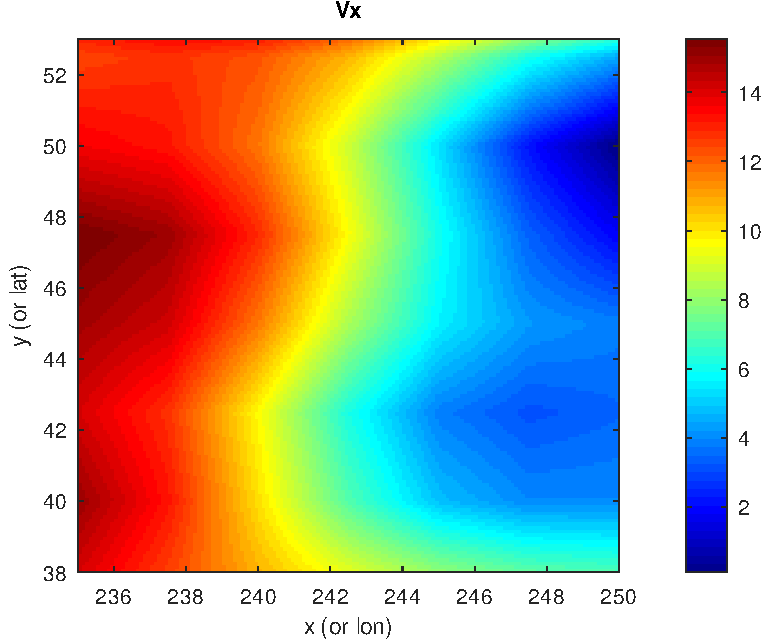
\includegraphics[angle=0,scale=0.55]{Figs/RegNCEP.pdf}
 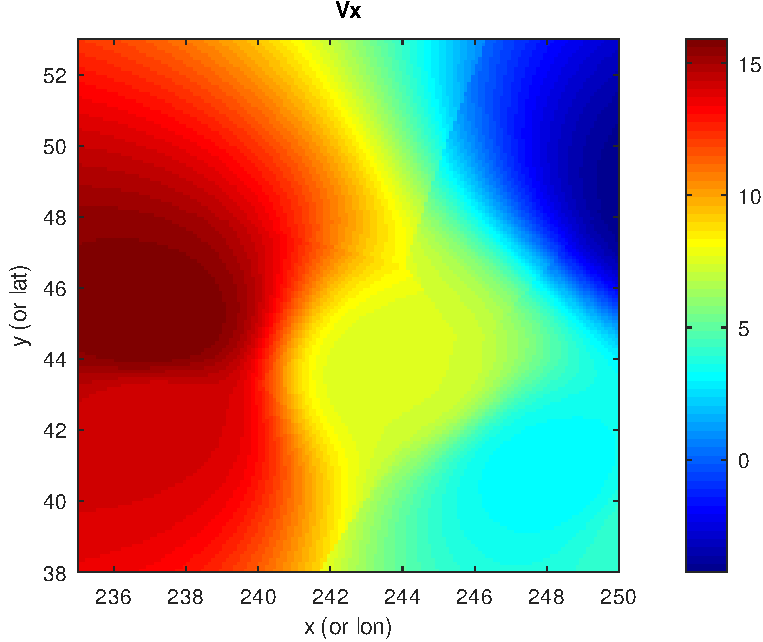
\includegraphics[angle=0,scale=0.55]{Figs/RegSonde.pdf}
 \parbox{15cm}{\caption{\label{FigRegrid}
 Example regridded output of $V_x$ of the NCEP reanalysis (\texttt{iwformat=25}) and
 6-point radiosonde data (left and right, respectively) using \texttt{RegridMet} with control files
 from the \texttt{examples} folder.
 }}
 \end{center}\end{figure}


\subsection{\texttt{MetSonde}}
This utility is used for probing the either GFS or NCEP 50-uear reanalysis files and
returning the temperature as a function of height.  
Usage:\\
\verb|  MetSonde lon lat YYYY MM DD HH [WIND_ROOT]|

The program assumes that the GFS and NCEP files are placed in the default directory, or
at least in default subdirectories off of \texttt{WIND\_ROOT}.  Values are interpolated
onto the requested point and time and are written to a file (\texttt{GFS\_prof.dat}) in
the current working directory.  This 3-column file contains the height (in $\mathrm{km}$),
pressure (in $\mathrm{Pa}$) and temperature (in $^{\circ}\mathrm{C}$).

\subsection{\texttt{MetProbe}}
This program is a more general version of \texttt{MetSonde}, requiring 15 or more command-line
arguments.  The command-line arguments are as follows.
\\
\begin{tabular}{ l  l  l }
filename      & string    & name of input file \\
timestep      & integer   & time step in file \\
llflag        & integer   & 0 for using windfile grid; 1 for forcing Lat/Lon \\
lon/x         & real      & longitude (or x) of sonde point \\
lat/y         & real      & latitude (or y) of sonde point \\
trunc flag    & character & truncation flag (T or F) \\
nvars         & integer   & number of pressure variables to export \\
varID(nvars)  & integers  & variable ID's to read and export (Tab \ref{ApVar}) \\
iw            & integer   & windfile format code (3,4,5) \\
iwf           & integer   & windfile product code \\
idf           & integer   & igrid (2 for nc, 3 for grib) \\
year          & integer   & only needed for iw = 5 files \\
month         & integer   & only needed for iw = 5 files \\
day           & integer   & only needed for iw = 5 files \\
hour          & real      & only needed for iw = 5 files \\
\end{tabular}

For example, the following command will probe a GFS file and write out
GPH, U, V, and T.

\verb| MetProbe 2020061000_5.f006.nc 1 0 190.055 52.8222 T 4 1 2 3 5 4 20 2 |

This will write output data to the file \texttt{NWP\_prof.dat}.
If the truncation flag is set to \texttt{T}, then data are not interpolated onto
the requested point, but instead the data corresponding to the node of the NWP
grid on the lower-left of the cell containing the point will be writen to the output file.

\subsection{\texttt{MetTraj}}

This utility takes a similar argument list as \texttt{MetSonde}, but instead of
probing a single point and time, this utility calculates trajectories within
the NWP files.
This utility must be compiled with either a \texttt{-DFORWARD} or \texttt{-DBACKWARD}
preprocessor flag to generate separate executables for forward or backward trajectories.
This utility can be run with a limited set of command-line arguments if GFS or NCEP
reanalysis data are to be used, or using a control file which can be used to specify
a more exhaustive set of options.

For the command-line options, \texttt{MetTraj\_[F,B]} requires at least the longitude,
latitude, year, month, day and hour.  Optionally, the simulation time (in hours) can
be provided (default is 24).  Additionally, the trajectory levels can be provided,
first with the number of
levels, followed by the level altitudes in km.  To specify 6 hours
integrations at 3 levels (5, 10, and 15 km), use:

\verb|MetTraj_[F,B] -169.9468 52.8217 2022 8 29 5.5 6.0 3 5.0 10.0 15.0 |

If levels are not provided, then 6 levels are assumed at heights of 1.52,
3.05, 6.10, 9.14, 12.19, 15.24 km; corresponding to 5000, 10000, 20000, 30000,
40000, and 50000 ft.

The location of the windfiles is assumed to be the default for GFS and NCEP.
To test for the optimal windfiles to use, \texttt{MetTraj\_[F,B]} uses three
parameters that describe the GFS windfiles.
\texttt{FC\_freq} (default = 12 hours) is the frequency that the GFS forecast
packages are downloaded.  
\texttt{GFS\_Archive\_Days} (default = 14 days) is the number of days the GFS
forecast packages are stored on the system.
\texttt{GFS\_FC\_TotHours} (default = 198 hours) is the number of forecast hours
downloaded for each forecast package.
For  forward trajectories, forecast package beginning most closely prior to the requested
start time is used unless the start time is greater than two weeks from present.  If
so, the NCEP files are used.  For the backward trajectories, the forecast package
chosen is that which can accommodate the default 24-hours of backward integration.

For each of the trajectory calculations, files are written to the current working directory
with the longitude and latitude of the trajectory in 1-hour increments at various
elevations.  The default elevations are 5000, 10000, 20000, 30000, 40000, and
50000 $\mathrm{ft}$.  Files for forward trajectories are named \texttt{ftraj[1-6].dat}
while the backward trajectories are  \texttt{btraj[1-6].dat}.

Optionally, the length of time to integrate and a user-specified list of output
elevations can be given.  Elevations are given on the command line must be in
$\mathrm{km}$.

Usage:\\
\verb|  MetTraj_F lon lat YYYY MM DD HH [FC_hours nlev lev1 lev2 ...]|

If a single string command-line argument if given, it is interpreted to be a control
file. The control file has the following format.

\footnotesize
\begin{verbatim}
-122.18 46.20                         ! lon lat
1980 5 18 15.5                        ! YYYY MM DD HH.H
24.0                                  ! simtime
1                                     ! streamflag (0 for streak, 1 for streamlines)
60                                    ! output time step (minutes)
6                                     ! ntraj (<10)
1.524 3.048 6.096 9.144 12.192 15.240 ! level values in km
1 4 -107.0 50.0 50.0 50.0 6367.470    ! Output projection
5 25 2 2                              ! iwind iwindformat igrid iformat
0 12 14                               ! autoflag (0 for auto, 1 for specified) FC_freq GFS_Archive_Days
1                                     ! number of windfiles
NCEP
\end{verbatim}
\normalsize

The first two lines specify the start point in space and time.  Line 3 gives the length of time
in hours for the trajectory forecast.  Note that GPH values at the start point are
used throughout the simulation so longer simulation times will lead to greater errors in
assumed GPH values.  Line 4 is an integer flag specifying streamlines (1) where the winds
evolve in time along the trajectory, or streakline (0) where a static initial wind
field is used.
Line 5 allows users to specify the output interval in minutes (default is 60).  Line 6
is the number of output trajectory levels (up to 10).  In line 7, the altitudes of
these trajectories is specified.
Line 8 specifies the coordinate system of the output grid.
Line 9 gives the windfile descriptions (\texttt{iwind iwindformat igrid iformat}).
Line 10 allows windfiles to be spelected automatically, similar to when this utility
is run with command-line options only.  Alternatively, line 11 will specify the number
of windfiles to read, followed by the windfile names in lines 12+.
Examples of several command files are given in the folder, \texttt{examples} with some
select output shown in Figure \ref{FigTraj}
\begin{figure}[htbp]\begin{center}
 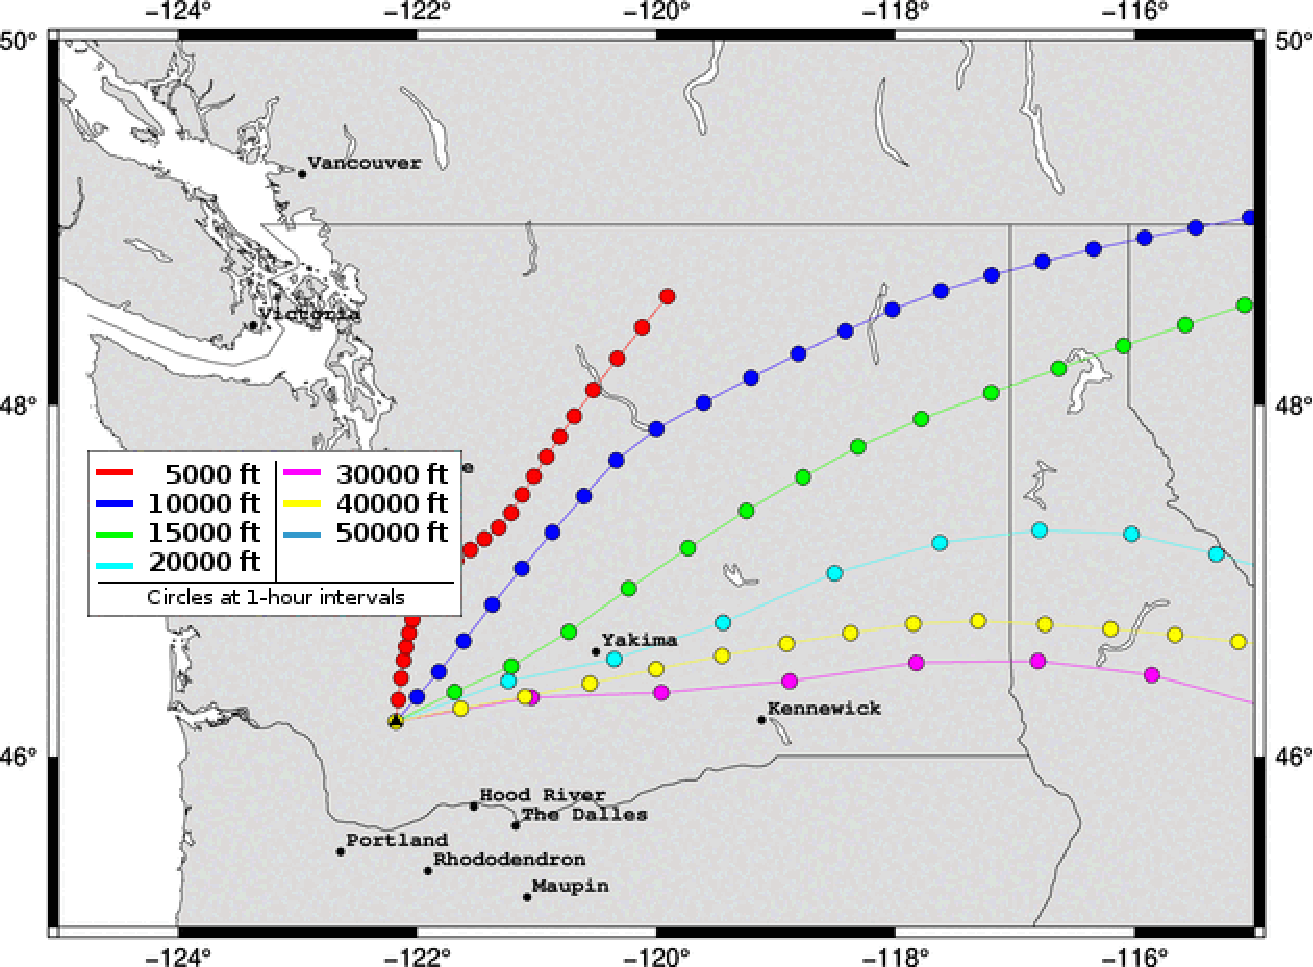
\includegraphics[angle=0,scale=0.3]{Figs/trajectory_NCEP.pdf}
 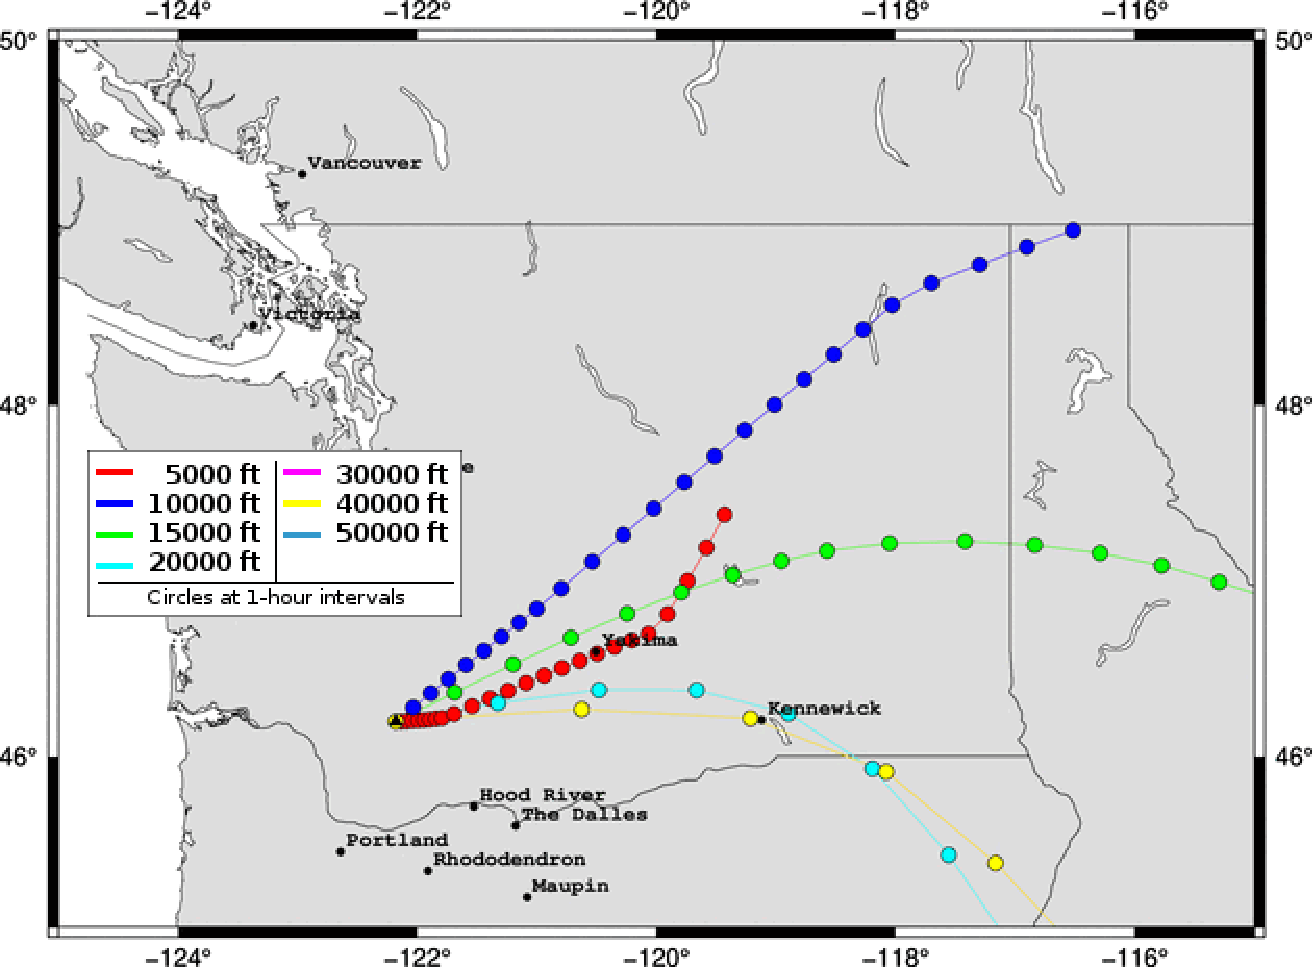
\includegraphics[angle=0,scale=0.3]{Figs/trajectory_Sonde.pdf}
 \parbox{15cm}{\caption{\label{FigTraj}
 Example of foreward trajectory output using NCEP reanalysis (\texttt{iwformat=25}) and
 6-point radiosonde data (left and right, respectively) using \texttt{RegridMet} with control files
 from the \texttt{examples} folder.  The start time for both these trajectory simulations is
 May 18, 1980, 15:30 UTC. Because \texttt{MR\_iHeightHandler=2} by default, the trajectories for 30,000
 and 40,000 ft for the radiosonde data are equivalent.
 }}
 \end{center}\end{figure}

\subsection{\texttt{makegfsncml}}
This utility generates a \texttt{ncml} file that can be used when converting
grib files to netcdf.  The \texttt{ncml} provides tthe conversion tool a template
for identifying which variables to exclued when writing the netcdf file.

\section{Windfile management scripts}
Scripts used to manage GFS and NCEP Reanalysis files are provided in the
folder \texttt{autorun\_scripts}.
The script \texttt{autorun\_gfs0.5deg\_00} (and the dependent scripts
\texttt{get\_gfs0.5deg.sh} and\\
\texttt{convert\_gfs0.5deg.sh}) is used for downloading and
converting the $0.5^{\circ}$ GFS files from NCEP.  This script is intended to be
run from a cron job and take as a parameter, the hour of the forecast package.  For example
\texttt{autorun\_gfs0.5deg.sh 0} will download for 00Z for the current date.  These 
scripts use a default root download directory of \texttt{/data/WindFiles}, but this can
be modified within the scripts.  The GFS files will be downloaded to\\
\texttt{/data/WindFiles/gfs/gfs.YYYYMMDDHH} where \texttt{HH} is the forecast hour
(00, 06, 12, or 18).  The forecast files from hours 0-99 are downloaded then converted using
netcdf-java 4.5.  The path this package is set to \texttt{~/ncj/netcdfAll-4.5.jar} but can be
modified in \texttt{convert\_gfs0.5deg.sh}.

Similarly, the script \texttt{get\_NCEP\_50YearReanalysis.sh} manages the downloading of 
the NCEP reanalysis files.  These are placed in \texttt{/data/WindFiles/NCEP/YYYY/}

These scripts are intended to be run as cron jobs.  The following line can be added to the
crontab to download the files once they are available.
\footnotesize
\begin{verbatim}
01 22 * * *   /opt/USGS/bin/autorun_scripts/autorun_gfs.sh 0p50 0  > gfs00_log 2>&1
01 11 * * *   /opt/USGS/bin/autorun_scripts/autorun_gfs.sh 0p50 12 > gfs12_log 2>&1
01 01 * * Sun /opt/USGS/bin/autorun_scripts/autorun_NCEP_50YearReanalysis.sh > NCEP_50yr_log   2>&1
\end{verbatim}
\normalsize

Also included in \texttt{autorun\_scripts} is a simple stand-alone script (\texttt{grib2nc.sh})
for converting GRIB files to NetCDF using \texttt{netcdf-java}.

\clearpage

\section{Appendix}
\subsection{Variable codes}\label{ApVar}
\begin{table}[h]\label{TabVar}
\caption{Variable codes}
\small
\begin{tabular}{| r | l | l | l |}
\hline
Variable type & ID & Name & dimensions \\
\hline
\multirow{7}{*}{3-D Mechanical} 
 &  1 & Geopotential Height & $\mathrm{gmp}$ or $\mathrm{m^2/s^2}$ \\
 &  2 & Vx & $\mathrm{m/s}$ \\
 &  3 & Vy & $\mathrm{m/s}$ \\
 &  4 & Vz & $\mathrm{Pa/s}$ \\
 &  5 & Temperature  & $\mathrm{K}$ \\
 &  6 & Wind speed & $\mathrm{m/s}$ \\
 &  7 & Wind direction &deg East of North \\
\hline
\multirow{10}{*}{Surface}
 &  10 & Planetary Boundary Layer Height & $\mathrm{m}$ \\
 &  11 & U @ 10m & $\mathrm{m/s}$ \\
 &  12 & V @ 10m & $\mathrm{m/s}$ \\
 &  13 & Friction velocity & $\mathrm{m/s}$ \\
 &  14 & Displacement Height & $\mathrm{m}$ \\
 &  15 & Snow depth & \% \\
 &  16 & Soil moisture & $\mathrm{kg/m2}$ \\
 &  17 & Surface Roughness & $\mathrm{m}$ \\
 &  18 & Wind gust speed & $\mathrm{m/s}$ \\
 &  19 & surface temperature & $\mathrm{K}$ \\
\hline
\multirow{6}{*}{Atmospheric Structure}
 &  20 & pressure at lower cloud base & $\mathrm{Pa}$ \\
 &  21 & pressure at lower cloud top & $\mathrm{Pa}$ \\
 &  22 & temperature at lower cloud top & $\mathrm{K}$ \\
 &  23 & Total Cloud cover & \% \\
 &  24 & Cloud cover (low) & \% \\
 &  25 & Cloud cover (convective) & \% \\
\hline
\multirow{4}{*}{Moisture}
  & 30 & Rel. Hum & \% \\
  & 31 & QV (specific humidity) & $\mathrm{kg/kg}$ \\
  & 32 & QL (liquid) & $\mathrm{kg/kg}$ \\
  & 33 & QI (ice) & $\mathrm{kg/kg}$ \\
\hline
\multirow{8}{*}{Precipitation}
  & 40 & Categorical rain & 0 or 1 \\
  & 41 & Categorical snow & 0 or 1 \\
  & 42 & Categorical frozen rain & 0 or 1 \\
  & 43 & Categorical ice & 0 or 1 \\
  & 44 & Precipitation rate large-scale (liquid) & $\mathrm{kg/m^2s}$ \\
  & 45 & Precipitation rate convective  (liquid) & $\mathrm{kg/m^2s}$ \\
  & 46 & Precipitation rate large-scale (ice) & $\mathrm{kg/m^2s}$ \\
  & 47 & Precipitation rate convective  (ice) & $\mathrm{kg/m^2s}$ \\
\hline
\end{tabular}
\normalsize
\end{table}

\clearpage
\subsection{NWP product ID (\texttt{iwf})}\label{Apiwf}
Several NWP product (both reanalysis and forecast) are recognized
and do not need template files.  These are listed in the table below
by the format code.  \texttt{iwf=1,2} are ASCII files.
\texttt{iwf=3-19} are reserved for products with projected grids.
\texttt{iwf=20-49} are reserved for global (lon/lat) grids.
\texttt{iwf=50} is for NetCDF output from Weather Research and 
Forecasting (WRF) simulations.

\begin{table}[h]\label{Tabiwf}
\caption{NWP product ID}
\begin{tabular}{| r | l | l | l |}
\hline
iwf & Product & NCEP Grid & resolution \\
\hline
  0 & Custom format based on template & & \\
  1 & ASCII profile & & \\
  2 & Radiosonde data & & \\
\hline
  3 & North American Regional Reanalysis NARR & 221 & 32 km \\
  4 & NAM Regional North America & 221 & 32 km \\
  5 & NAM Regional Alaska & 216 & 45 km \\
  6 & NAM N. Hemisphere & 104 & 90 km \\
  7 & NAM Regional CONUS & 212 & 40 km \\
  8 & NAM Regional CONUS & 218 & 12 km \\
  9 & NAM Regional CONUS & 227 & 5.08 km \\
 10 & NAM Regional Alaska & 242 & 11.25 km \\
 11 & NAM Regional Hawaii & 196 & 2.5 km \\
 12 & NAM Regional Alaska & 198 & 5.953 km \\
 13 & NAM Regional Alaska & 91 & 2.976 km \\
 14 & NAM Regional CONUS & None & 3.0 km \\
\hline
 20 & GFS & 4   & $ 0.5 \, ^{\circ}$ \\
 21 & GFS & 3   & $ 1.0 \, ^{\circ}$ \\
 22 & GFS & 193 & $0.25 \, ^{\circ}$ \\
 23 & NCEP-DOE Reanalysis 2 & 2  & $2.5 \, ^{\circ}$ \\
 24 & NASA-MERRA-2 Reanalysis & None & $0.625 \, \times \,0.5^{\circ}$ \\
 25 & NCEP/NCAR Reanalysis 1 & 2 & $2.5 \, ^{\circ}$ \\
 26 & JRA-55 & 45 & $1.25 \, ^{\circ}$ \\
 27 & NOAA-CIRES 20th Century Reanalysis & 2 & $2.5^{\circ}$ \\
 28 & ECMWF ERA-Interim Reanalysis & 170 & $\sim 0.7^{\circ}$-Gaussian \\
 29 & ECMWF ERA5 Reanalysis & None & $0.281$ \\
 30 & ECMWF ERA-20C Reanalysis & None & $1.125 \, \times \, \sim 1.121^{\circ}$-Gaussian\\
\hline
 32 & Air Force Weather Agency subcenter = 0 & None & $0.25^{\circ}$ \\
 33 & CCSM3.0 Community Atmosphere Model &None & $3.75 \, \times \,3.7^{\circ}$\\
\hline
 40 & NASA GEOS-5 Cp & None & $0.625 \, \times \,0.5^{\circ}$ \\
 41 & NASA GEOS-5 Np & None & $0.3125 \, \times \,0.25^{\circ}$\\
 50 & WRF - output & None & \\
\hline
\end{tabular}
\end{table}
\clearpage
\subsection{Example Template files}\label{ApTemplate}
\begin{figure}[htbp]\begin{center}
 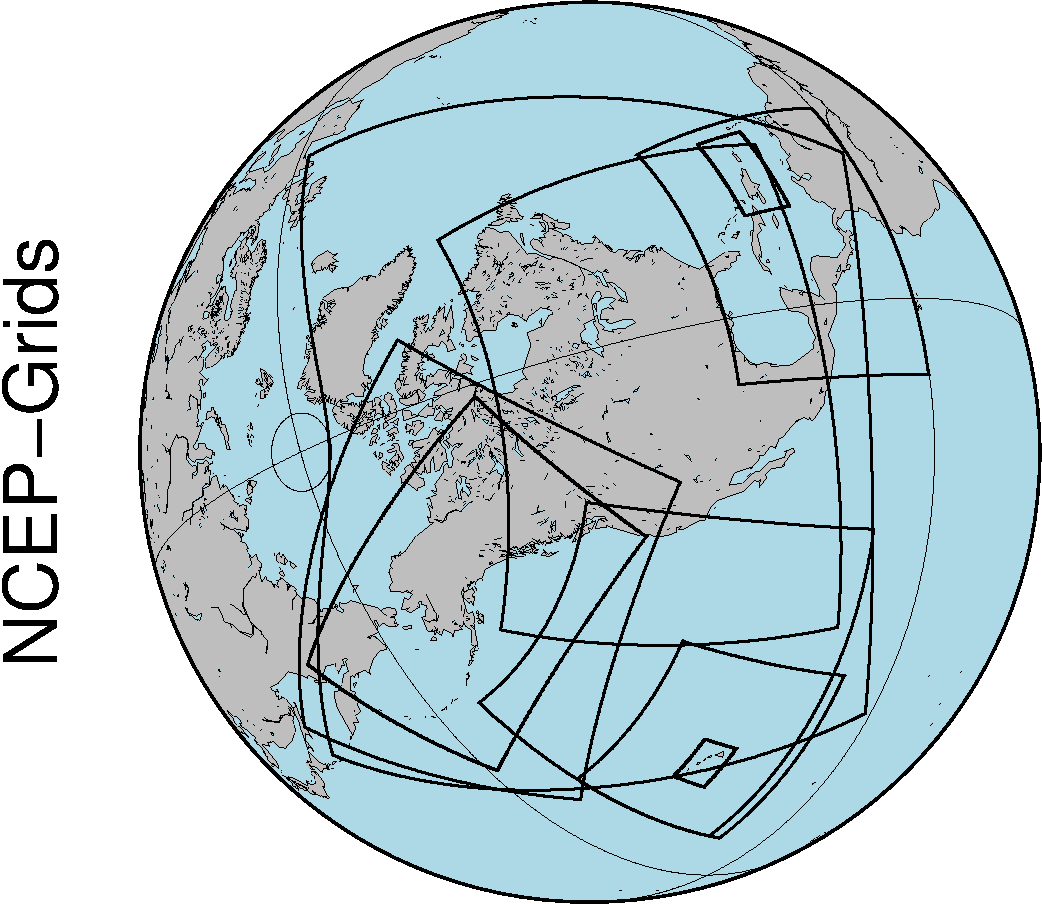
\includegraphics[angle=-90,scale=0.7]{Figs/Overview_NCEP-Grids.pdf}
\parbox{15cm}{\caption{\label{FigNAMs}
Outlines of North America Mesoscale (NAM) and Global Forecast System (GFS)
models from NCEP that are compatible with MetReader template files.
}}
\end{center}\end{figure}

%%%%%%%%%%%%%%%%%%%%%%%%%%%%%%%%%%%%%%%%%%%%%%%%%%%%
% Broader North America
%%%%%%%%%%%%%%%%%%%%%%%%%%%%%%%%%%%%%%
%\clearpage
%\subsection{NAM 5 Regional N.America (190.5 km)}
%
%  NOTE:  This requires a general stereographic projection.
%         libproj.a only provides polar stereographic
%
%\verb|nam.t00z.grb5fm00.tm00|\\
%Available from:\\
%\verb|ftp://ftp.ncep.noaa.gov/pub/data/nccf/com/nam/prod/nam.YYYYMDD/| \\
%
%\begin{figure}[htbp]\begin{center}
% \includegraphics[angle=-90,scale=0.9]{Figs/n005.pdf}
%\parbox{15cm}{\caption{\label{FigNAM005}
%NAM 5, Regional N. America 190.5 km Polar Stereographic
%}}
%\end{center}\end{figure}
%\clearpage
%\verb|n005_template.txt| \\
%\tiny \verbatiminput{n005_template.txt} \normalsize


%%%%%%%%%%%%%%%%%%%%%%%%%%%%%%%%%%%%%%
%\clearpage
%\subsection{NAM 104 Regional N.America (90.7 km)}
%  NOTE:  Corners of this grid extend beyond the horizon causing errors with GMT.
%         These regions are NaN's in the data.
%
%\verb|nam.t00z.grbgrd00.tm00|\\
%Available from:\\
%\verb|ftp://ftp.ncep.noaa.gov/pub/data/nccf/com/nam/prod/nam.YYYYMDD/| \\
%
%\begin{figure}[htbp]\begin{center}
%% \includegraphics[angle=-90,scale=0.5]{Figs/grid104.pdf}
%\parbox{15cm}{\caption{\label{FigNAM005}
%NAM 104, Regional N. America 90.7 km Polar Stereographic
%}}
%\end{center}\end{figure}
%\clearpage
%\verb|n104_template.txt| \\
%\tiny \verbatiminput{n104_template.txt} \normalsize


%%%%%%%%%%%%%%%%%%%%%%%%%%%%%%%%%%%%%%
\clearpage
\subsection{NAM 221 Regional N.America (32.5 km)}

\verb|nam.t00z.awip3200.tm00|\\
Available from:\\
\verb|ftp://ftp.ncep.noaa.gov/pub/data/nccf/com/nam/prod/nam.YYYYMDD/| \\

\begin{figure}[htbp]\begin{center}
 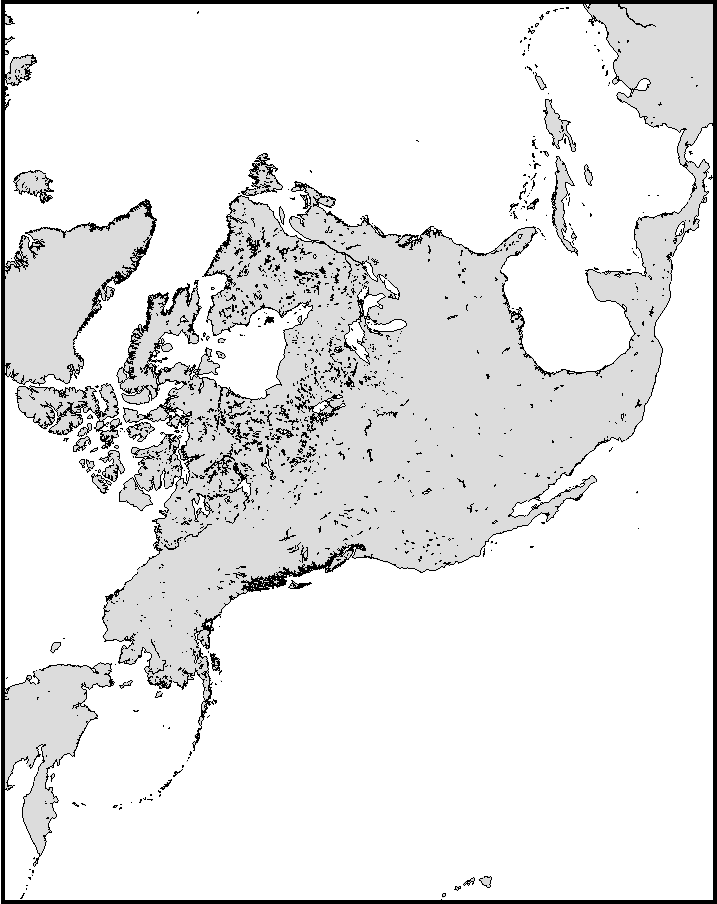
\includegraphics[angle=-90,scale=1.0]{Figs/n221.pdf}
\parbox{15cm}{\caption{\label{FigNAM221}
NAM 221, Regional N. America 32.5 km Lambert Conformal Conical
}}
\end{center}\end{figure}
\clearpage
\verb|n221_template.txt| \\
\tiny \verbatiminput{n221_template.txt} \normalsize


%%%%%%%%%%%%%%%%%%%%%%%%%%%%%%%%%%%%%%
% Alaska
%%%%%%%%%%%%%%%%%%%%%%%%%%%%%%%%%%%%%%
\clearpage
\subsection{NAM 216 AK (45.0 km); NAM 242 AK (11.25 km)}

\verb|nam.t00z.awipak00.tm00|\\
Available from:\\
\verb|ftp://ftp.ncep.noaa.gov/pub/data/nccf/com/nam/prod/nam.YYYYMDD/| \\
\verb|http://motherlode.ucar.edu/native/conduit/data/nccf/com/nam/prod/nam.YYYYMMDD/|\\

\begin{figure}[htbp]\begin{center}
 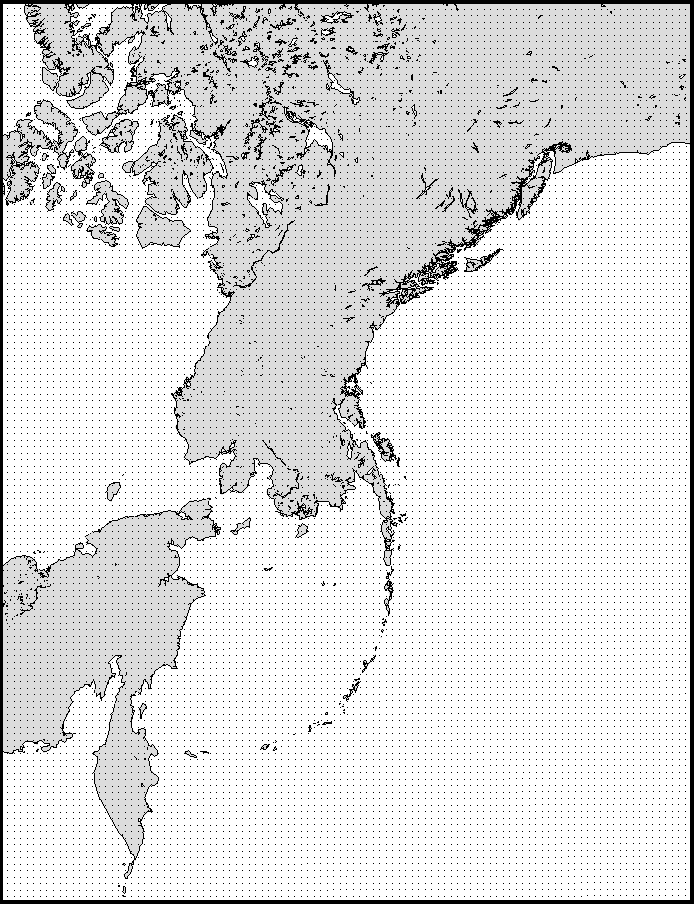
\includegraphics[angle=-90,scale=1.0]{Figs/n216.pdf}
\parbox{15cm}{\caption{\label{FigNAM2116}
NAM 216, AK 45.0 km Polar Stereographic
}}
\end{center}\end{figure}
\clearpage 
\verb|n216_template.txt| \\
\tiny \verbatiminput{n216_template.txt} \normalsize


%%%%%%%%%%%%%%%%%%%%%%%%%%%%%%%%%%%%%%
\clearpage
%\subsection{NAM 242 AK (11.25km)}
Grid 242 uses the same projection and domain as Grid 216, but with 11.25 km
grid spacing.

\verb|nam.t00z.awak3d00.grb2.tm00|\\
Available from:\\
\verb|ftp://ftp.ncep.noaa.gov/pub/data/nccf/com/nam/prod/nam.YYYYMDD/|

%\begin{figure}[htbp]\begin{center}
% \includegraphics[angle=-90,scale=1.0]{Figs/n242.pdf}
%\parbox{15cm}{\caption{\label{FigNAM242}
%NAM 242, AK 11.25 km Polar Stereographic
%}}
%\end{center}\end{figure}
%\clearpage 
\verb|n242_template.txt| \\
\tiny \verbatiminput{n242_template.txt} \normalsize

%%%%%%%%%%%%%%%%%%%%%%%%%%%%%%%%%%%%%%
\clearpage
\subsection{NAM 91 AK (2.95 km); NAM 198 AK (5.9 km)}

\verb|nam.t00z.alaskanest.hiresf00.tm00|\\
Available from:\\
\verb|ftp://ftp.ncep.noaa.gov/pub/data/nccf/com/nam/prod/nam.YYYYMDD/| \\

\begin{figure}[htbp]\begin{center}
 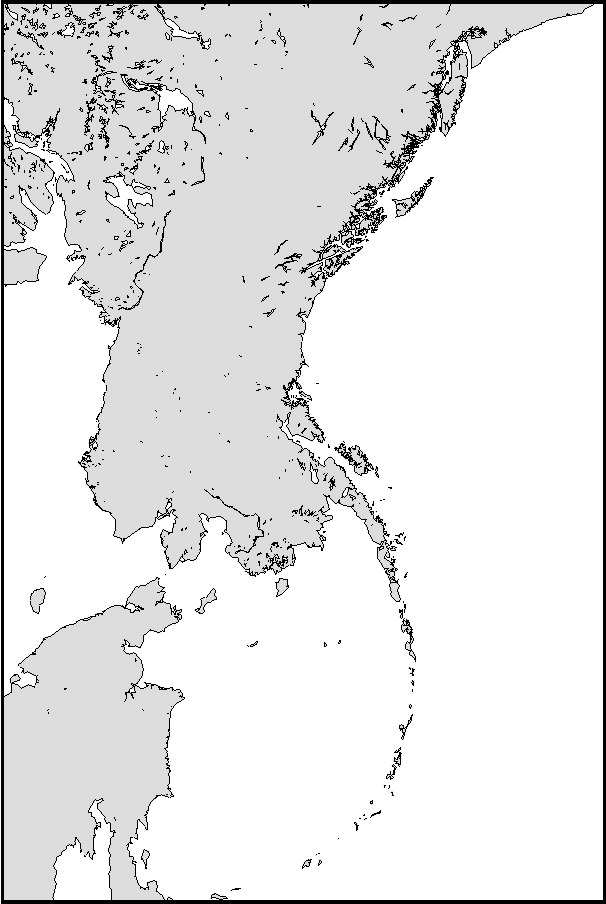
\includegraphics[angle=-90,scale=1.0]{Figs/n091.pdf}
\parbox{15cm}{\caption{\label{FigNAM198}
NAM 91, AK 2.95 km Polar Stereographic (previously NAM 198, AK 5.9 km)
}}
\end{center}\end{figure}
\clearpage
\verb|n091_template.txt| \\
\tiny \verbatiminput{n091_template.txt} \normalsize


%%%%%%%%%%%%%%%%%%%%%%%%%%%%%%%%%%%%%%
% North Pacific / Hawaii
%%%%%%%%%%%%%%%%%%%%%%%%%%%%%%%%%%%%%%
\clearpage
\subsection{NAM 243 Eastern N. Pac./HI ($0.40  \, ^{\circ}$)}

\verb|nam.t00z.awiphi00.tm00|\\
Available from:\\
\verb|ftp://ftp.ncep.noaa.gov/pub/data/nccf/com/nam/prod/nam.YYYYMDD/|

\begin{figure}[htbp]\begin{center}
 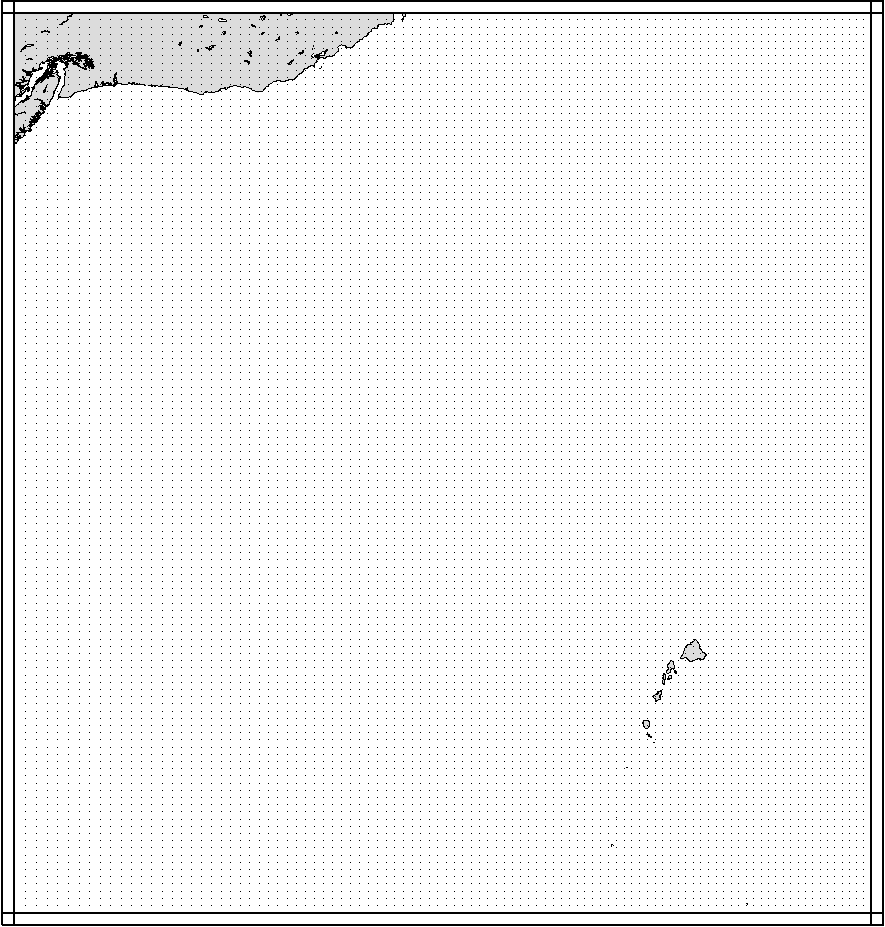
\includegraphics[angle=-90,scale=0.9]{Figs/n243.pdf}
\parbox{15cm}{\caption{\label{FigNAM243}
NAM 243, Eastern N. Pac./HI $0.4 \, ^{\circ}$
}}
\end{center}\end{figure}
\clearpage
\verb|n243_template.txt| \\
\tiny \verbatiminput{n243_template.txt} \normalsize

%%%%%%%%%%%%%%%%%%%%%%%%%%%%%%%%%%%%%%
\clearpage
\subsection{NAM 182 HI ($0.108  \, ^{\circ}$)}

\verb|nam.t00z.afwahi00.grb2.tm00|\\
Available from:\\
\verb|ftp://ftp.ncep.noaa.gov/pub/data/nccf/com/nam/prod/nam.YYYYMDD/|

\begin{figure}[htbp]\begin{center}
 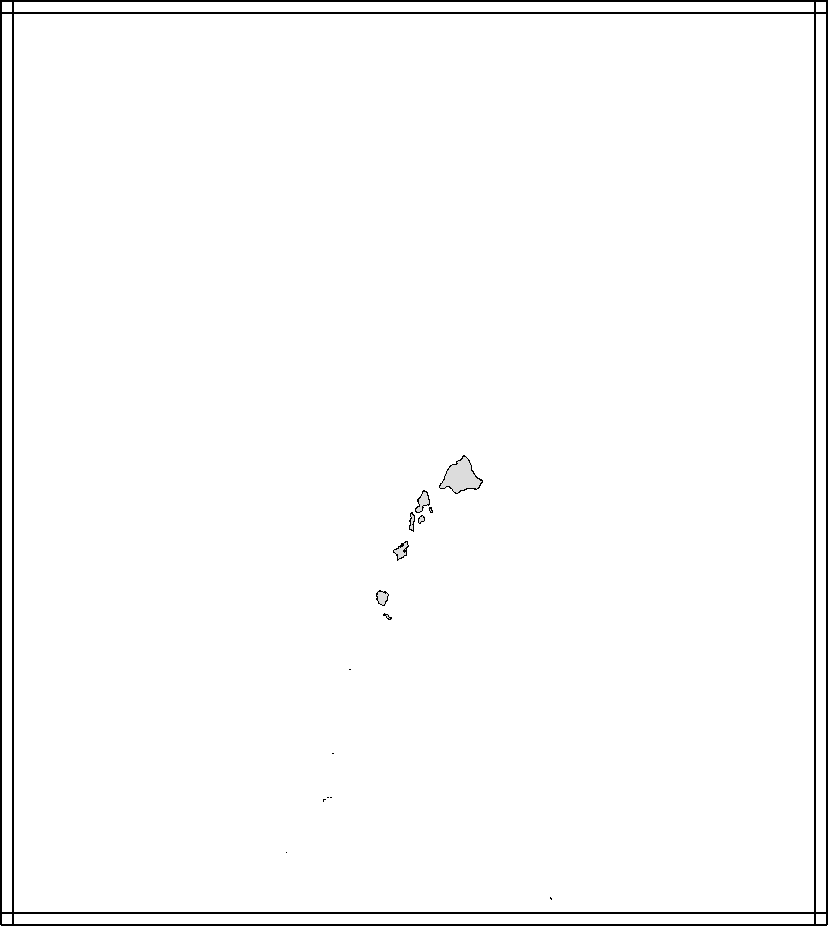
\includegraphics[angle=-90,scale=0.9]{Figs/n182.pdf}
\parbox{15cm}{\caption{\label{FigNAM182}
NAM 182, HI $0.108  \, ^{\circ}$
}}
\end{center}\end{figure}
\clearpage
\verb|n182_template.txt| \\
\tiny \verbatiminput{n182_template.txt} \normalsize


%%%%%%%%%%%%%%%%%%%%%%%%%%%%%%%%%%%%%%
\clearpage
\subsection{NAM 196 HI (2.5 km)}

\verb|nam.t00z.hawaiinest.hiresf00.tm0|\\
Available from:\\
\verb|ftp://ftp.ncep.noaa.gov/pub/data/nccf/com/nam/prod/nam.YYYYMDD/|

\begin{figure}[htbp]\begin{center}
 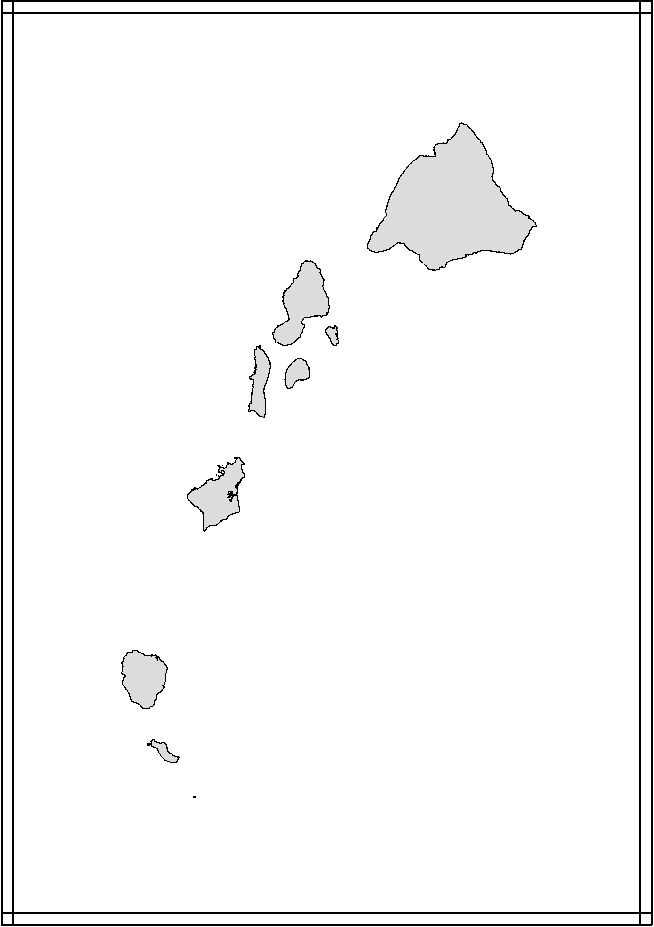
\includegraphics[angle=-90,scale=1.0]{Figs/n196.pdf}
\parbox{15cm}{\caption{\label{FigNAM196}
NAM 196, AK 2.5 km Mercator
}}
\end{center}\end{figure}
\clearpage
\verb|n196_template.txt| \\
\tiny \verbatiminput{n196_template.txt} \normalsize

%%%%%%%%%%%%%%%%%%%%%%%%%%%%%%%%%%%%%%
% Continental U.S.
%%%%%%%%%%%%%%%%%%%%%%%%%%%%%%%%%%%%%%
\clearpage
\subsection{NAM 211/212/218/227 CONUS}

\begin{figure}[htbp]\begin{center}
 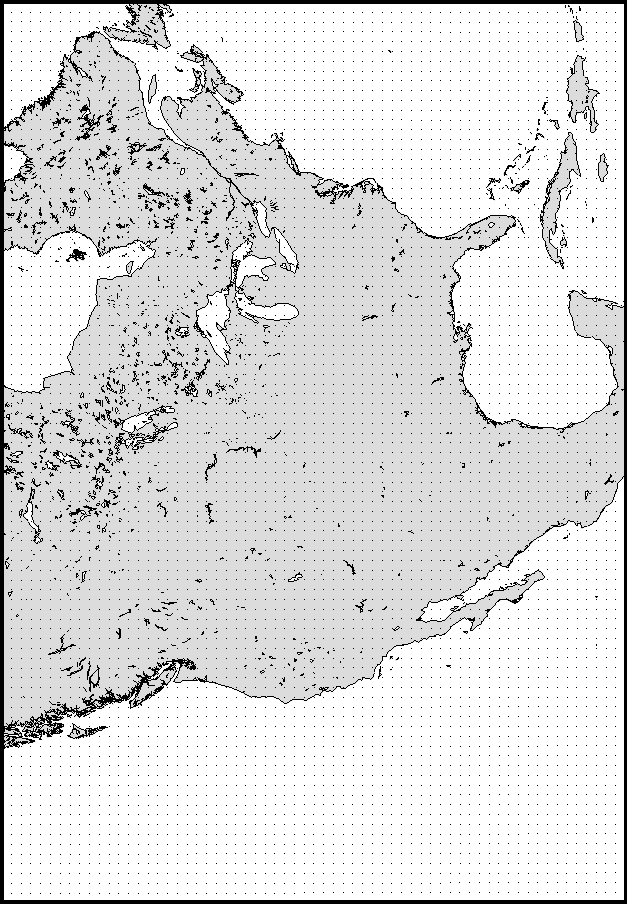
\includegraphics[angle=-90,scale=1.0]{Figs/n211.pdf}
\parbox{15cm}{\caption{\label{FigNAM211}
NAM 211/212/218/227 CONUS Lambert Conformal Conical (dots
correspond to the 81.3 km 211 grid)
}}
\end{center}\end{figure}
\clearpage

Available from:\\
\verb|ftp://ftp.ncep.noaa.gov/pub/data/nccf/com/nam/prod/nam.YYYYMDD/|

NAM 211 CONUS (81.3 km) :: \verb|nam.t00z.awp21100.tm00|\\
\verb|n211_template.txt| \\
\tiny \verbatiminput{n211_template.txt} \normalsize

NAM 212 CONUS (40.6 km) :: \verb|nam.t00z.awip3d00.tm00|\\
\verb|n212_template.txt| \\
\tiny \verbatiminput{n212_template.txt} \normalsize

NAM 218 CONUS (12.2 km) :: \verb|nam.t00z.awphys00.grb2.tm00|\\
\verb|n218_template.txt| \\
\tiny \verbatiminput{n218_template.txt} \normalsize

NAM 227 CONUS (5.1 km)  :: \verb|nam.t00z.conusnest.hiresf00.tm00|\\
\verb|n227_template.txt| \\
\tiny \verbatiminput{n227_template.txt} \normalsize

%%%%%%%%%%%%%%%%%%%%%%%%%%%%%%%%%%%%%%
% Eastern U.S, / Caribbean
%%%%%%%%%%%%%%%%%%%%%%%%%%%%%%%%%%%%%%
\clearpage
\subsection{NAM 181 Caribbean ($0.108  \, ^{\circ}$)}

\verb|nam.t00z.afwaca00.grb2.tm00|\\
Available from:\\
\verb|ftp://ftp.ncep.noaa.gov/pub/data/nccf/com/nam/prod/nam.YYYYMDD/|

\begin{figure}[htbp]\begin{center}
 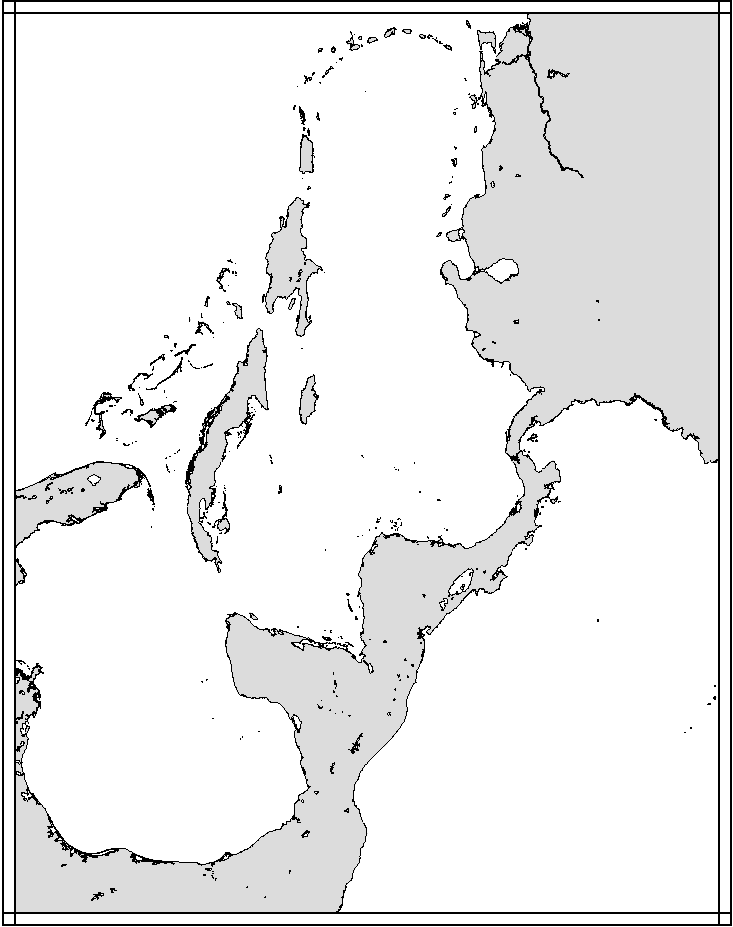
\includegraphics[angle=-90,scale=0.9]{Figs/n181.pdf}
\parbox{15cm}{\caption{\label{FigNAM181}
NAM 181, Caribbean $0.108  \, ^{\circ}$
}}
\end{center}\end{figure}
\clearpage
\verb|n181_template.txt| \\
\tiny \verbatiminput{n181_template.txt} \normalsize


%%%%%%%%%%%%%%%%%%%%%%%%%%%%%%%%%%%%%%
% Global 
%%%%%%%%%%%%%%%%%%%%%%%%%%%%%%%%%%%%%%
\clearpage
\subsection{GFS 3/4/193}

\begin{figure}[htbp]\begin{center}
 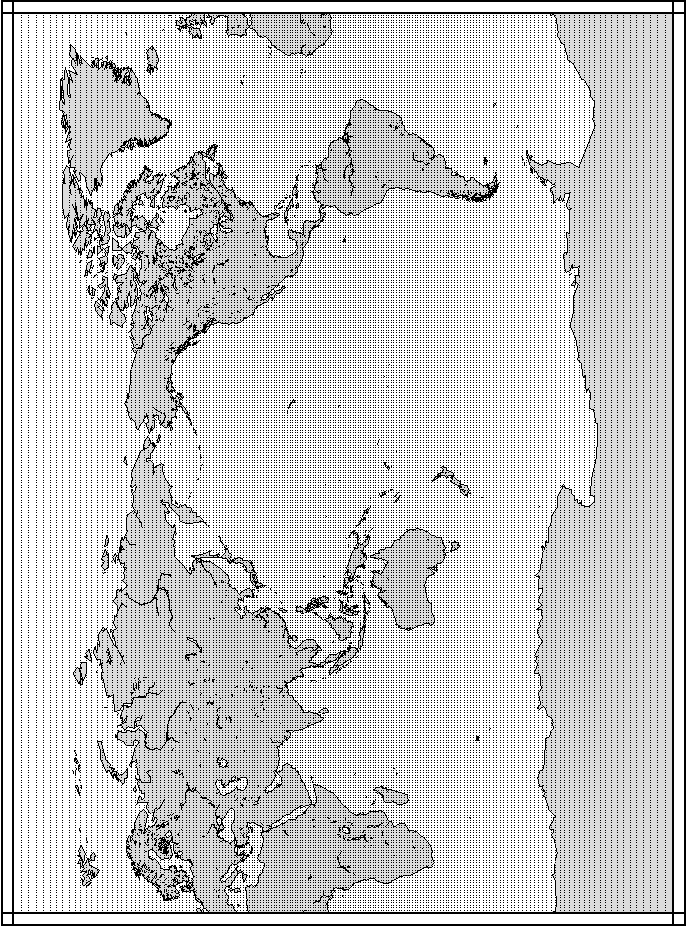
\includegraphics[angle=0,scale=0.95]{Figs/n003.pdf}
\parbox{15cm}{\caption{\label{FigNAM003}
GFS 3,4,193, (dots correspond to the $1.0 \, ^{\circ}$ NAM 3 grid)
}}
\end{center}\end{figure}
\clearpage

Available from:\\
\verb|ftp://ftp.ncep.noaa.gov/pub/data/nccf/com/gfs/prod/gfs.YYYYMDD/|

GFS NCEP Grid 3 ($1.0  \, ^{\circ}$) :: \verb|gfs.t00z.pgrb2.1p00.f000.nc|\\
\verb|n003_template.txt| \\
\tiny \verbatiminput{n003_template.txt} \normalsize

GFS NCEP grid 4 ($0.5 \, ^{\circ}$) :: \verb|n004_template.txt| \\
\tiny \verbatiminput{n004_template.txt} \normalsize

GFS NCEP grid 193 ($0.25 \, ^{\circ}$) :: \verb|n193_template.txt| \\
\tiny \verbatiminput{n193_template.txt} \normalsize

%%%%%%%%%%%%%%%%%%%%%%%%%%%%%%%%%%%%%%
\clearpage
\subsection{NASA GEOS-5}

\begin{figure}[htbp]\begin{center}
 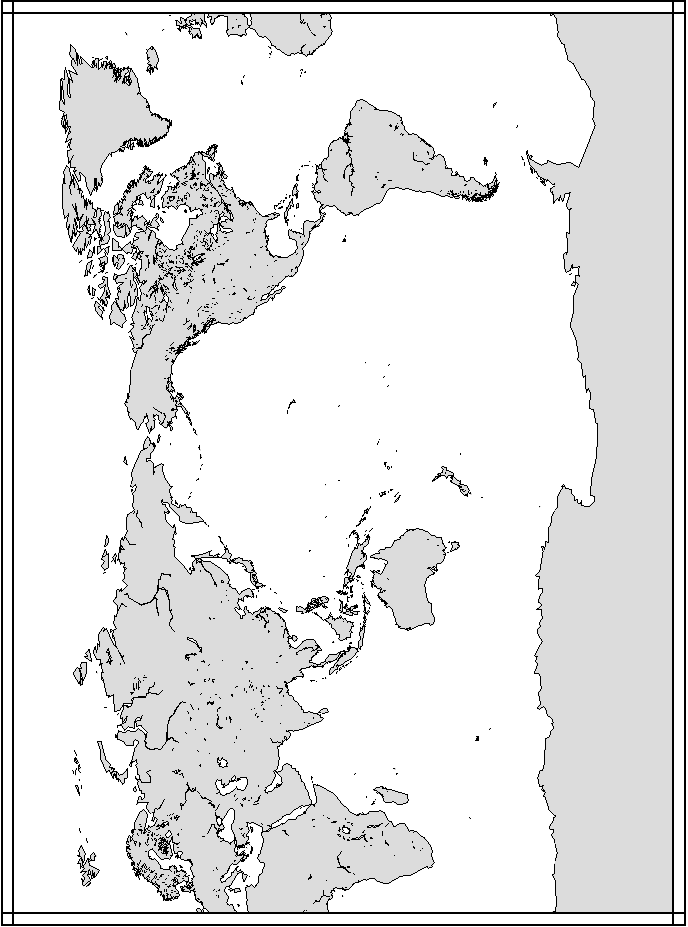
\includegraphics[angle=0,scale=0.95]{Figs/nGCp.pdf}
\parbox{15cm}{\caption{\label{FigGCp}
NASA GEOS-5, $0.625/0.5 \, ^{\circ}$
}}
\end{center}\end{figure}
\clearpage

Available from:\\
\verb|ftp://gmao_ops@ftp.nccs.nasa.gov/fp/forecast//|

NASA GEOS-5 Cp ($0.625/0.5  \, ^{\circ}$) :: \\
\verb|GEOS.fp.fcst.inst3_3d_asm_Cp.YYYYMMDD_00+YYYYMMDD_mmmm.V01.nc4|\\
\verb|nGCp_template.txt| \\
\tiny \verbatiminput{nGCp_template.txt} \normalsize

NASA GEOS-5 Np ($0.25/0.3125  \, ^{\circ}$) :: \\
\verb|GEOS.fp.fcst.inst3_3d_asm_Np.YYYYMMDD_00+YYYYMMDD_mmmm.V01.nc4|\\
\verb|nGNp_template.txt| \\
\tiny \verbatiminput{nGNp_template.txt} \normalsize

%
%NCEP
%  REFTIME  => time(attribute='units')="Hour since 2016-01-25T00:00:00Z"
%  STEPTIME => time(i) = double hours
%
%	double time(time) ;
%		time:units = "Hour since 2016-01-25T00:00:00Z" ;
%		time:standard_name = "time" ;
%		time:long_name = "GRIB forecast or observation time" ;
%Catania
%  REFTIME  => reftime="2015 03 25 00:0"
%  STEPTIME => frtime(i) = float hours
%
%	float frtime(frtime) ;
%		frtime:units = "hours" ;
%	char reftime(timelen) ;
%             reftime = "2015 03 25 00:00" ;
%
%
%
%NASA
%  REFTIME  => time(attribute='units')="minutes since 2016-01-25 03:00:00"
%  STEPTIME => time(i) = integer minutes
%
%	int time(time) ;
%		time:long_name = "time" ;
%		time:units = "minutes since 2016-01-25 03:00:00" ;
%		time:time_increment = 30000 ;
%		time:begin_date = 20160125 ;
%		time:begin_time = 30000 ;
%		time:vmax = 1.e+15f ;
%		time:vmin = -1.e+15f ;
%		time:valid_range = -1.e+15f, 1.e+15f ;
%        double TIME_EOSGRID(TIME_EOSGRID) ;
%                TIME_EOSGRID:hdf_name = "TIME:EOSGRID" ;
%                TIME_EOSGRID:begin_time = 0 ;
%                TIME_EOSGRID:begin_date = 20150721 ;
%                TIME_EOSGRID:time_increment = 30000 ;
%                TIME_EOSGRID:units = "minutes since 2015-07-21 00:00:00" ;
%                TIME_EOSGRID:long_name = "time" ;
%
%
%UM
%  REFTIME  => time(attribute='units')="hours since 2015-11-04T12:00:00Z"
%  STEPTIME => time(i) = int hours
%
%        int time(time) ;
%                time:long_name = "forecast time" ;
%                time:units = "hours since 2015-11-04T12:00:00Z" ;
%                time:GRIB_orgReferenceTime = "2015-11-04T12:00:00Z" ;
%                time:GRIB2_significanceOfRTName = "Start of forecast" ;
%                time:_CoordinateAxisType = "Time" ;
%
%STEPTIME=time double or int
%         frtime float
%REFTIME=time:units  "..YYYY.MM.DD.HH.MM.SS"
%        reftime

\end{document}
